\chapterimage{chap35.jpg}
\chapter{Summary}
1. $\lim\limits_{x\rightarrow +\infty}\frac{\sqrt{x+\sqrt{x+\sqrt{x}}}}{\sqrt{x+1}}$
\begin{solution}
	
	原极限等价于:  
	$$\lim\limits_{x\rightarrow 0}\frac{x+\sqrt{x+\sqrt{x}}}{x+1}=1\Rightarrow \text{原极限为}1$$
\end{solution}
2. $\lim\limits_{n\rightarrow +\infty}n[(1+\frac{x}{n})^n-e^x]$
\begin{solution}
	
	原极限等价于:  
	$$\lim\limits_{n\rightarrow +\infty}n[e^{nln(1+\frac{x}{n})}-e^x]=\lim\limits_{n\rightarrow +\infty}n[e^{n\frac{x}{n}}-e^x]=0$$
\end{solution}
3. $\lim\limits_{x\rightarrow 0}x^{x^{x}-1}$
\begin{solution}
	
	原极限等价于:  
	$$\lim\limits_{x\rightarrow 0}e^{(e^{xlnx}-1)ln x}=\lim\limits_{x\rightarrow 0}e^{xln^2 x}=1$$
\end{solution}
4.双曲函数
\begin{figure}[htbp]
	\centering
	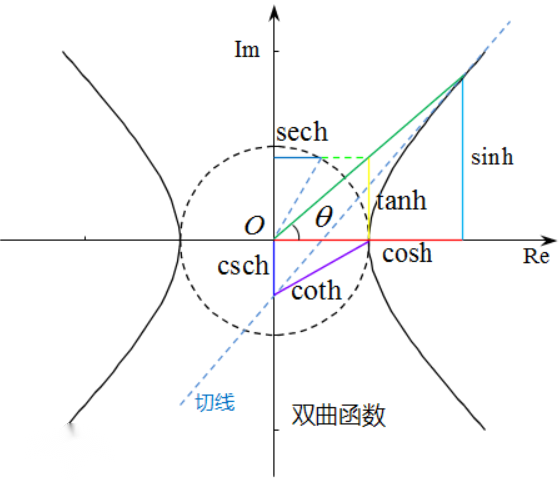
\includegraphics[width=9.5cm,height=8cm]{"figure/Summary/双曲函数.png"}
\end{figure} 
\begin{definition}\label{def: 双曲函数}
	双曲函数是一种类似于三角函数的一类函数,基本的函数有双曲正弦函数和双曲余弦函数,借由指数函数定义.
	
	1. 双曲正弦函数 
	$$\sinh x=\frac{e^{x}-e^{-x}}{2},x\in \mathbb{R}\quad \mathbb{R}\rightarrow \mathbb{R}$$
	
	2. 双曲余弦函数
	$$\cosh x=\frac{e^{x}+e^{-x}}{2},x\in \mathbb{R}\quad \mathbb{R}\rightarrow [1,+\infty]$$
	
	3. 双曲正切函数
	$$\tanh x=\frac{e^{x}-e^{-x}}{e^{x}+e^{-x}},x\in \mathbb{R}\quad \mathbb{R}\rightarrow (-1,1)$$
	
	恒等式:  
	$$\cosh^2 x-\sinh^2=1$$
	$$\sinh x=-i\sin ix,\quad \cosh x=\cos ix$$
	$$\sinh x=\sum\limits_{n=0}^{+\infty}\frac{x^{2n+1}}{(2n+1)!}=x+\frac{x^3}{3!}+\frac{x^5}{5!}+\dots$$
	$$\cosh x=\sum\limits_{n=0}^{+\infty}\frac{x^{2n}}{2n!}=1+\frac{x^2}{2!}+\frac{x^4}{4!}+\dots$$
\end{definition}
\begin{definition}
	反双曲函数:  
	
	1. 反双曲正弦函数
	$$\arsinh x=ln(x+\sqrt{x^2+1}),\quad (arsinh x)'=\frac{1}{\sqrt{x^2+1}}$$
	
	2. 反双曲余弦函数
	$$\arcosh x=ln(x+\sqrt{x^2-1}),\quad (arcosh x)'=\frac{1}{\sqrt{x^2-1}}$$
	
	3. 反双曲正切函数
	$$\artanh x=\frac{1}{2}ln(\frac{1+x}{1-x}),\quad (artanh x)'=\frac{1}{1-x^2}$$
\end{definition}
5 .$\int\dfrac{\arctan x}{x^2(1+x^2)}dx$
\begin{solution}
	
	原不定积分等价于:  
	$$\int\dfrac{\arctan x}{x^2}dx-\int\frac{\arctan x}{1+x^2}dx$$
	$$I_{1}=\int\arctan xd(-\frac{1}{x})=-\frac{\arctan x}{x}+\int\frac{1}{x(1+x^2)}dx=-\frac{\arctan x}{x}+\frac{1}{2}ln\frac{x^2}{1+x^2}$$
	$$I_{2}=\frac{1}{2}\arctan^{2}x$$
	
	原不定积分为:  $$\frac{1}{2}ln\frac{x^2}{1+x^2}-\frac{\arctan x}{x}-\frac{1}{2}\arctan^{2}x+C$$
\end{solution}
6. 设 $y=y(x)$ 在 $(-1,1)$ 二阶可导,满足方程 $(1-x^2)\frac{d^2 y}{d x^2}-x\frac{dy}{dx}+a^2y=0$,做变量替换$x=\sin t$后,$y$ 作为 $t$ 的函数满足的方程.
\begin{solution}
	
	$$\frac{dy}{dt}=\frac{dy}{dx}\frac{dx}{dt}=\frac{dy}{dx}\cos t,\quad \frac{d^2y}{dt^2}=\frac{d^2y}{dx^2}\cos^2 t-\frac{dy}{dx}\sin t $$
	我们得到:  
	$$\frac{dy}{dx}=\frac{1}{\cos t}\frac{dy}{dt},\quad \frac{d^2y}{dx^2}=\frac{1}{\cos^2 t}(\frac{d^2y}{dt^2}+\frac{dy}{dt}\frac{\sin t}{\cos t})$$
	
	新的方程为:  
	$$\frac{d^2y}{dt^2}+a^2y=0$$
\end{solution}

7. 曲率和曲率半径
\begin{definition}
	曲率是描述曲线的弯曲程度的量.
	
	$$k=\dfrac{|f''(x_{0})|}{[1+(f'(x_{0}))^{2}]^{\frac{3}{2}}}$$
	$$R=\dfrac{1}{k}=\dfrac{[1+(f'(x_{0}))^{2}]^{\frac{3}{2}}}{|f''(x_{0})|},(f''(x_{0})\neq 0)$$
	
\end{definition}

8. 心形线、摆线、三叶玫瑰线、星形线、伯努利曲线和阿基米德螺线
\begin{definition}\label{def: 常用曲线}
	几类特殊曲线的面积、弧长、旋转体体积
	
	1.心形线 \quad $r=a(1+\cos \theta)$
	$$L=\int_{0}^{2\pi}\sqrt{a^2(1+\cos \theta)^2+a^2\sin^2\theta}d\theta=8a$$
	$$S=2\int_{0}^{\pi}a^2(1+\cos \theta)^2d\theta=\frac{3}{2}a^2\pi$$
	
	2.摆线\quad 
	$\left\lbrace
	\begin{array}{l}
		x=a(\theta-\sin \theta)\\
		y=a(1-\cos \theta)
	\end{array}
	 \right. $
	 $$L=\int_{0}^{2\pi}\sqrt{a^2(1-\cos \theta)^2+a^2\sin^2\theta}d\theta=8a$$
	 $$S=\int_{0}^{x_{0}}f(x)dx=\int_{0}^{2\pi}a^2(1-\cos \theta)^2d\theta=3a^2\pi$$
	
	3.星形线\quad $x^{\frac{2}{3}}+y^{\frac{2}{3}}=a^{\frac{2}{3}}\Leftrightarrow$
	$\left\lbrace
	\begin{array}{l}
		x=a\cos^3\theta\\
		y=a\sin^3\theta
	\end{array}
	 \right. $
	$$L=4\int_{0}^{\frac{\pi}{2}}3a\sin\theta\cos\theta d\theta=6a$$
	$$S=4\int_{0}^{\frac{\pi}{2}}3a\sin^4\theta\cos^2\theta=\frac{3\pi}{8}a^2$$
	
	4.三叶玫瑰线 \quad $\rho=a\cos 3\theta$\quad $\rho=a\sin 3\theta$
	$$L=3\int_{\frac{\pi}{6}}^{\frac{\pi}{2}}\sqrt{a^2\cos^2 3\theta+9a^2\sin^2 3\theta}d\theta=2a\int_{0}^{\frac{\pi}{2}}\sqrt{1+8\sin^2 t}dt$$
	$$S=\frac{3}{2}\int_{\frac{\pi}{6}}^{\frac{\pi}{2}}a^2\cos^2 3\theta d\theta=\frac{\pi a^2}{4}$$
	
	5.伯努利双扭线\quad $\rho^2=a^2\cos 2\theta$
	$$L=4\int_{0}^{\frac{\pi}{4}}a\sqrt{\frac{\sin^2 2\theta}{\cos 2\theta}+\cos^2 2\theta}=2a\int_{0}^{\frac{\pi}{2}}\cos^{-\frac{1}{2}}\theta d\theta$$
	$$S=2\int_{0}^{\frac{\pi}{4}}a^2\cos 2\theta d\theta=a^2$$
\end{definition}
\begin{figure}[H]
	\centering  %图片全局居中
	\subfigure[心形线]{
	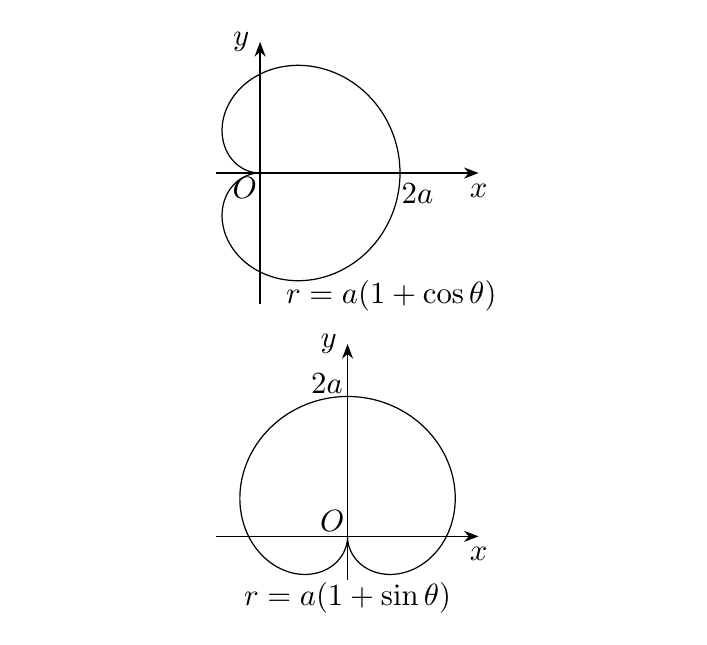
\includegraphics[width=0.45\textwidth]{"figure/Summary/心形线.png"}}
	\subfigure[摆线]{
	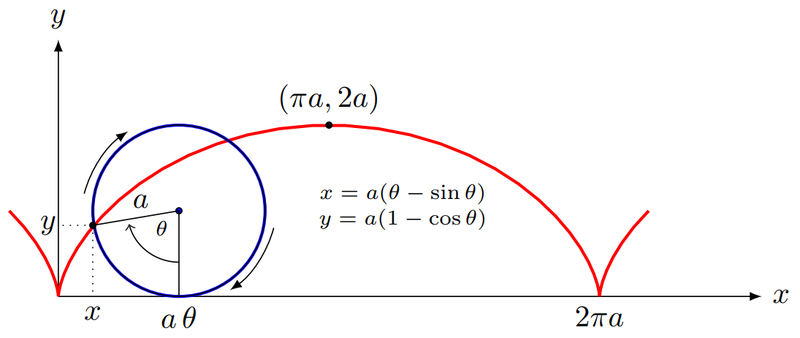
\includegraphics[width=0.45\textwidth]{"figure/Summary/摆线.png"}}
	\subfigure[星形线]{
	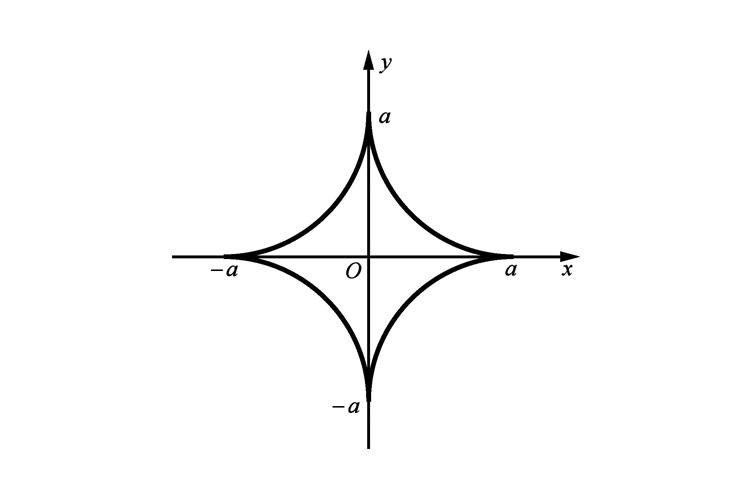
\includegraphics[width=0.45\textwidth]{"figure/Summary/星形线.jpg"}}
	\subfigure[三叶玫瑰线$\rho=a\cos 3\theta$]{
	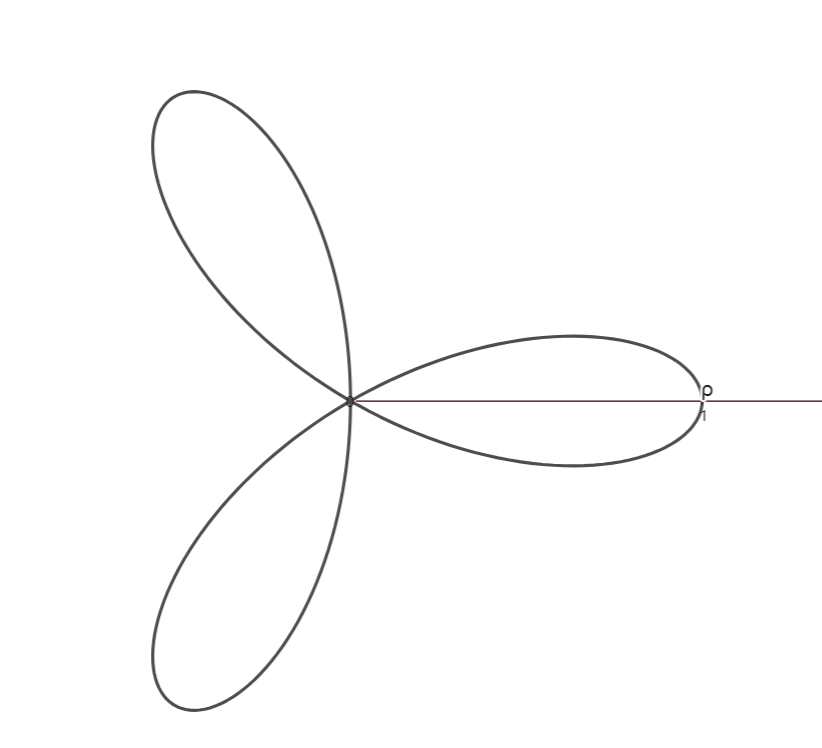
\includegraphics[width=0.45\textwidth]{"figure/Summary/三叶玫瑰线1.png"}}
	\subfigure[三叶玫瑰线$\rho=a\sin 3\theta$]{
	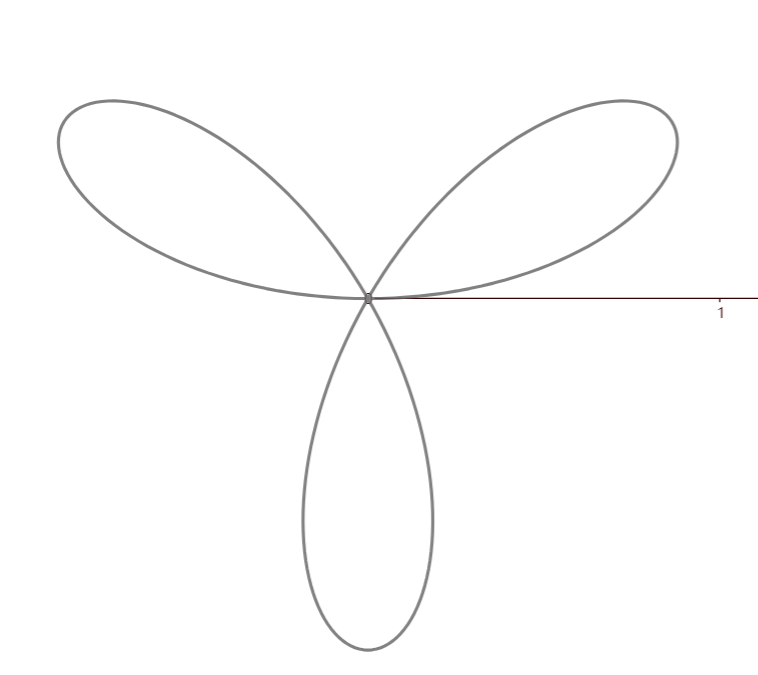
\includegraphics[width=0.45\textwidth]{"figure/Summary/三叶玫瑰线2.png"}}
	\subfigure[伯努利双扭线$\rho^2=a^2\cos 2\theta$]{
	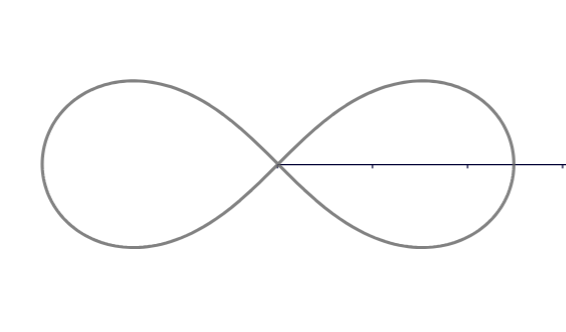
\includegraphics[width=0.45\textwidth]{"figure/Summary/伯努利双扭线.png"}}
	\caption{曲线图形}
\end{figure}
9. $Gamma$ 函数和 $Beta$函数
\begin{definition}[$Gamma$ 函数和 $Beta$函数]	
	1. $Gamma$ 函数(欧拉第一类积分)
	$$B(p,q)=\int_{0}^{1}x^{p-1}(1-x)^{q-1}dx=B(q,p)$$
	
	我们有:  $$B(a,b)=(\frac{x^a(1-x)^b}{a})|_{0}^{1}+\frac{b-1}{a}\int_{0}^{1}x^{a}(1-x)^{b-2}dx$$
	$$B(a,b)=\frac{b-1}{a}\int_{0}^{1}(x-1+1)x^{a-1}(1-x)^{b-2}$$
	$$\mathcolorbox{yellow}{B(a,b)=\frac{b-1}{a}[B(a,b-1)-B(a,b)]}$$ $$\mathcolorbox{yellow}{B(a,b)=\frac{b-1}{a+b-1}B(a,b-1)}$$
	
	特别的,我们有:  $$\mathcolorbox{yellow}{B(m,n)=\frac{(n-1)!(m-1)!}{(m+n-1)!}}$$
	
	2.$Beta$函数(第二类欧拉积分)
	$$\Gamma(\alpha)=\int_{0}^{+\infty}x^{\alpha-1}e^{-x}dx$$
	
	我们有:  $$\Gamma(\alpha)=(-x^{\alpha-1}e^{-x})|_{0}^{+\infty}+(\alpha-1)\int_{0}^{+\infty}x^{\alpha-2}e^{-x}dx$$
	$$\mathcolorbox{red}{\Gamma(\alpha)=(\alpha-1)\Gamma(\alpha-1)},\alpha>1$$
	
	特别的,我们有:  $$\mathcolorbox{red}{\Gamma(n+1)=n!}$$
	
	3. 两类积分之间的关系
	
	转换公式:  
	$$B(a,b)=\frac{\Gamma(a)\Gamma(b)}{\Gamma(a+b)}$$
	
\end{definition}
10. 常用极限技巧
\begin{theorem}\label{the: 常用极限技巧}
	(i).$\lim\limits_{n\rightarrow +\infty}\sqrt[n]{u_{1}^{n}+u_{2}^{n}+u_{3}^{n}+\cdots+u_{m}^{n}}=\text{max}\{ u_{1},u_{2},\cdots,u_{m}\}$
	
	证明:  $$\text{max}\{ u_{1},u_{2},\cdots,u_{m}\}\leq u_{1}^{n}+u_{2}^{n}+u_{3}^{n}+\cdots+u_{m}^{n}\leq m*\text{max}\{ u_{1},u_{2},\cdots,u_{m}\}$$
	我们将$\text{max}\{ u_{1},u_{2},\cdots,u_{m}\}$记作$a$,$m*\text{max}\{ u_{1},u_{2},\cdots,u_{m}\}$记作$b$,我们利用夹逼准则:  
	$$\lim\limits_{n\rightarrow +\infty}\sqrt[n]{a}=\lim\limits_{n\rightarrow +\infty}\sqrt[n]{b}=\text{max}\{ u_{1},u_{2},\cdots,u_{m}\}$$
\end{theorem}
11.变上限积分奇偶性、周期性和原函数关系
\begin{lemma}\label{lem: 变上限积分奇偶性和周期性与原函数关系}
	$f(x)$连续,$f(x)$与$\int_{a}^{x} f(t)dt$之间的关系
	
	(1).如果$f(x)$是奇函数,$\int_{a}^{x}f(t)dt$是偶函数
	
	(2).如果$f(x)$是偶函数,$\int_{a}^{x}f(t)dt$是奇函数当且仅当$a=0$时成立.
	
	(3).如果 $f(x)$ 是周期函数,$\int_{a}^{x}f(t)dt\text{是周期函数与}\int_{0}^{T}f(t)dt=0\text{等价}$
	
	\begin{eqnarray*}
		&&\text{证明:  我们令} F(x)=\int_{a}^{x}f(t)dt\\
		&&(i).\text{必要性:  } F(x+T)-F(x)=\int_{x}^{x+T}f(t)dt=\int_{0}^{T}f(t)dt=0\\
		&&(ii).\text{充分性:  }
		\int_{0}^{T}f(t)dt=0\Leftrightarrow F(x+T)-F(x)=0
	\end{eqnarray*}
\end{lemma}
12. 阿达玛不等式
\begin{figure}[htbp]
	\centering
	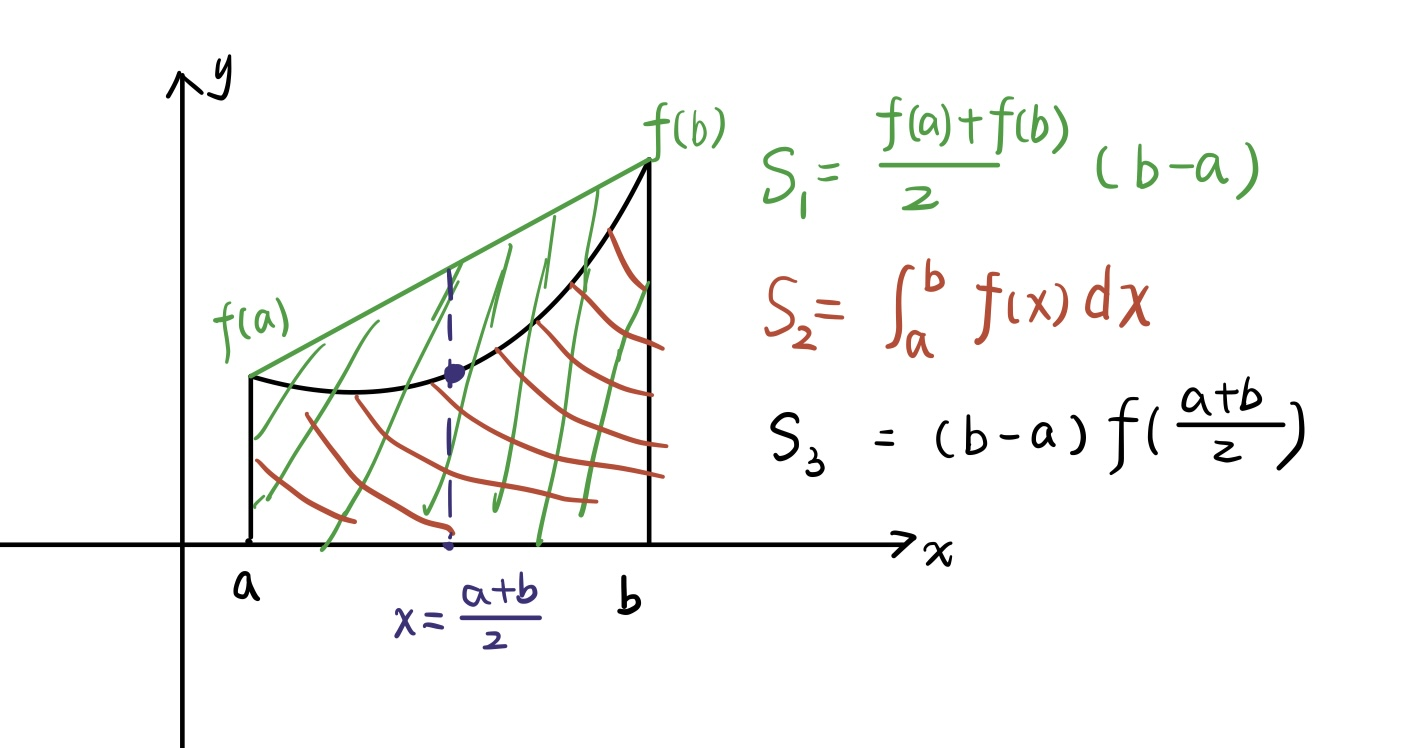
\includegraphics[width=15cm,height=8cm]{"figure/Summary/阿达玛不等式.jpg"}
	\caption{$Hadamard$不等式}
	\label{Figure: $Hadamard$不等式}
\end{figure} 
\begin{theorem}[$Hadamard$不等式]\label{thm: $Hadamard$不等式}
	$f(x)$在$[a,b]$上具有二阶导数,且$f''(x)\geq 0$,下面不等式成立:  
	$$f(\dfrac{a+b}{2})\leq \dfrac{1}{b-a}\int_{a}^{b}f(t)dt\leq \dfrac{1}{2}[f(a)+f(b)]$$
	\begin{proof}
		
		原不等式可以化为:  
		$$(b-a)f(\dfrac{a+b}{2})\leq\int_{a}^{b}f(t)dt\leq\dfrac{b-a}{2}[f(a)+f(b)]$$
		
		我们由图\ref{Figure: $Hadamard$不等式}可以发现:  
		
		不等式左边表示的过$(\dfrac{a+b}{2},f(\dfrac{a+b}{2}))$的切线与$x=a,x=b,y=0$围成的图形的面积$S_{3}$;
		
		不等式中间表示的是$f(x)$与$x=a,x=b,y=0$围成的曲边梯形的面积$S_{2}$;
		
		不等式右边表示的是直线$x=a,x=b,y=0$与直线$y=\dfrac{f(b)-f(a)}{b-a}(x-a)+f(a)$围成的梯形的面积$S_{1}$.
		
		我们可以由图形上直观的看出三个面积的大小关系:  $S_{3}\leq S_{2}\leq S_{1}$
		
		对于左边的不等式,我们将$f(x)$在$x=\dfrac{a+b}{2}$处展开得到:  
		$$f(x)=f(\dfrac{a+b}{2})+f'(\dfrac{a+b}{2})(x-\dfrac{a+b}{2})+f''(\xi)(x-\dfrac{a+b}{2})^2$$
		
		我们由$f''(x)>0$,我们可以得到:  
		$$f(x)>f(\dfrac{a+b}{2})+f'(\dfrac{a+b}{2})(x-\dfrac{a+b}{2})$$
		
		两边同时在$[a,b]$内取定积分得到:  
		$$\int_{a}^{b}f(x)dx>\int_{a}^{b}[f(\dfrac{a+b}{2})+f'(\dfrac{a+b}{2})(x-\dfrac{a+b}{2})]=(b-a)f(\dfrac{a+b}{2})$$
		
		对于右边的不等式,我们构造辅助函数:  
		$$F(x)=\dfrac{x-a}{2}[f(x)+f(a)]-\int_{a}^{x}f(t)dt,\ F(a)=0$$
		$$\left\lbrace
		\begin{array}{l}
			F'(x)=\dfrac{x-a}{2}f'(x)-\dfrac{f(x)-f(a)}{2}\\
			F''(x)=\dfrac{x-a}{2}f''(x)
		\end{array}
		\right. F'(0)=0,F''(x)\geq 0\Rightarrow F'(x)\geq 0$$
		
		我们得到$F'(x)\geq 0\Rightarrow F(x)\text{单调递增}$,$F(x)\geq F(a)=0$
	\end{proof}
\end{theorem}
13.$\lim\limits_{n\rightarrow +\infty}\dfrac{x_{n+1}}{x_{n}}\text{相关命题}$
\begin{theorem}[极限推论]
	1. $\lim\limits_{n\rightarrow +\infty}x_{n}=a$
	
	(i). $a\neq 0\Rightarrow \lim\limits_{n\rightarrow +\infty}\dfrac{x_{n+1}}{x_{n}}=1$
	
	(ii). $a=0\Rightarrow \lim\limits_{n\rightarrow +\infty}\dfrac{x_{n+1}}{x_{n}} \text{不一定存在}$
	
	2. $\lim\limits_{n\rightarrow +\infty}\dfrac{x_{n+1}}{x_{n}}=a$
	
	$$\left\lbrace 
	\begin{array}{l}
		\lim\limits_{n\rightarrow +\infty}x_{n}=\infty \text{当}|a|>1\\
		\lim\limits_{n\rightarrow +\infty}x_{n}=0,\text{当}|a|<1\\
		\lim\limits_{n\rightarrow +\infty}x_{n}\text{不确定},\text{当}|a|=1
	\end{array}
	\right. $$
	
	3. $\lim\limits_{n\rightarrow +\infty}\dfrac{x_{n+1}}{x_{n}}\text{存在且}x_{n}>0$,我们有:  
	$$\lim\limits_{n\rightarrow +\infty}\sqrt[n]{x_{n}}=\lim\limits_{n\rightarrow +\infty}\dfrac{x_{n+1}}{x_{n}}$$
\end{theorem}

14. 反函数导数公式
\begin{theorem}[反函数导数公式]\label{the: 反函数导数公式}
	$f(x)$的反函数$\varphi(y)$,我们有:  
	
	(1). $$\varphi'(y)=\dfrac{1}{f'(x)}$$
	
	(2). $$\varphi''(y)=\dfrac{d\varphi'(y)}{dx}\dfrac{dx}{dy}=-\dfrac{f''(x)}{[f'(x)]^3}$$
	
	(3)当$\left\lbrace 
	\begin{array}{l}
		x=\alpha(t)\\
		y=\beta(t)
	\end{array}
	\right. $,我们有:  
	$$\dfrac{dy}{dx}=\dfrac{dy}{dt}\dfrac{dt}{dx}=\dfrac{\beta'(t)}{\alpha'(t)}$$
	$$\dfrac{d^2y}{dx^2}=\dfrac{d(\frac{dy}{dx})}{dx}=\dfrac{d(\frac{\beta'(t)}{\alpha'(t)})}{dt}\dfrac{dt}{dx}=\dfrac{\beta''(t)\alpha'(t)-\alpha''(t)\beta'(t)}{[\alpha'(t)]^3}$$
\end{theorem}

15. 设$f(x)$为连续函数,$\varphi$为常数,$\int_{0}^{2\pi}f(\sin(x+\varphi))dx=A\int_{-\frac{\pi}{2}}^{\frac{\pi}{2}}f(\sin x)dx$,求$A$.
\myspace{1}
\begin{solution}
	
	我们得到函数$f(\sin x)$是周期函数,我们可以得到:  
	$$\int_{0}^{2\pi}f(\sin(x+\varphi))dx\overset{t=x+\varphi}{=}\int_{\varphi}^{2\pi+\varphi}f(\sin t)dt=\int_{-\frac{\pi}{2}}^{\frac{3\pi}{2}}f(\sin t)dt$$
	$$\int_{-\frac{\pi}{2}}^{\frac{3\pi}{2}}f(\sin t)dt=\int_{-\frac{\pi}{2}}^{\frac{\pi}{2}}f(\sin t)dt+\int_{\frac{\pi}{2}}^{\frac{3\pi}{2}}f(\sin t)dt$$
	\begin{eqnarray*}
		\int_{\frac{\pi}{2}}^{\frac{3\pi}{2}}f(\sin t)dt\overset{t=\pi-u}{=}\int_{-\frac{\pi}{2}}^{\frac{\pi}{2}}f(\sin u)du
	\end{eqnarray*}

	我们得到:  $$\int_{0}^{2\pi}f(\sin(x+\varphi))dx=2\int_{-\frac{\pi}{2}}^{\frac{\pi}{2}}f(\sin t)dt\Rightarrow A=2$$
\end{solution}
\begin{anymark}[注]
	[题目来源]:  $660 \ P_{61}$
\end{anymark}
\myspace{1}

16.设$D=\{(x,y)|-1\leq x\leq 1,\ 0\leq y\leq 2\}$,则$I=\iint\limits_{D}\sqrt{|y-x^2|}dxdy$
\myspace{1}
\begin{solution}
	
	原二重积分等价于:  
	\begin{eqnarray*}
		I&=&2[\iint\limits_{D_{1}}\sqrt{|y-x^2|}dxdy]\\
		 &=&2[\iint\limits_{D_{2}}\sqrt{y-x^2}dxdy+\iint\limits_{D_{3}}\sqrt{x^2-y}dxdy]\\
		 &=&2[\int_{0}^{1}dx\int_{x^2}^{2}\sqrt{y-x^2}dy+\int_{0}^{1}dx\int_{0}^{x^2}\sqrt{x^2-y}dy]\\
		 &=&2[\int_{0}^{1}\frac{2}{3}(2-x^2)^{\frac{3}{2}}dx+\int_{0}^{1}\frac{2}{3}x^3dx]\\
		 &=&\dfrac{4}{3}\int_{0}^{1}(2-x^2)^{\frac{3}{2}}dx+\dfrac{4}{3}\int_{0}^{1}x^3dx\\
		 &\overset{\text{三角换元}}{=}&\dfrac{16}{3}\int_{0}^{\frac{\pi}{4}}\cos^4 \theta d\theta+\dfrac{1}{3}\\
		 &=&\dfrac{\pi}{2}+\dfrac{5}{3}
	\end{eqnarray*}
\end{solution}
\begin{anymark}[注]
	[题目来源]:  $660 \ P_{116}$
\end{anymark}
\myspace{1}

17.证明函数$f(x)=3\arccos x-\arccos (3x-4x^3)$在$[-\dfrac{1}{2},\dfrac{1}{2}]$上恒为常数.
\myspace{1}
\begin{solution}
	
	我们对$f(x)$求导可得:  
	\begin{eqnarray*}
		f'(x)&=&-\dfrac{3}{\sqrt{1-x^2}}+\dfrac{3-12x^2}{\sqrt{1-(3x-4x^3)^2}}\\
		&=&-\dfrac{3}{\sqrt{1-x^2}}+\dfrac{3-12x^2}{\sqrt{(1+3x-4x^3)(1-3x+4x^3)}}\\
		&=&-\dfrac{3}{\sqrt{1-x^2}}+\dfrac{3-12x^2}{\sqrt{(1-x)(1+2x)^2(1+x)(2x-1)^2}}\\
		&=&-\dfrac{3}{\sqrt{1-x^2}}+\dfrac{3-12x^2}{(1-4x^2)\sqrt{1-x^2}}\\
		&=&0
	\end{eqnarray*}

	我们由$f'(x)=0\Rightarrow f(x)=C$
\end{solution}
\begin{anymark}[注]
	[题目来源]:  $660 \ P_{172}$
\end{anymark}
\myspace{1}

18.设$L$是连接两点$A(0,1)$与$B(1,0)$的一条凸弧,$P(x,y)$是$L$上任意一点,已知凸弧$L$与弦$AP$围成的平面图形的面积等于$x^4$,求$L$的方程.
\begin{figure}[htbp]
	\centering
	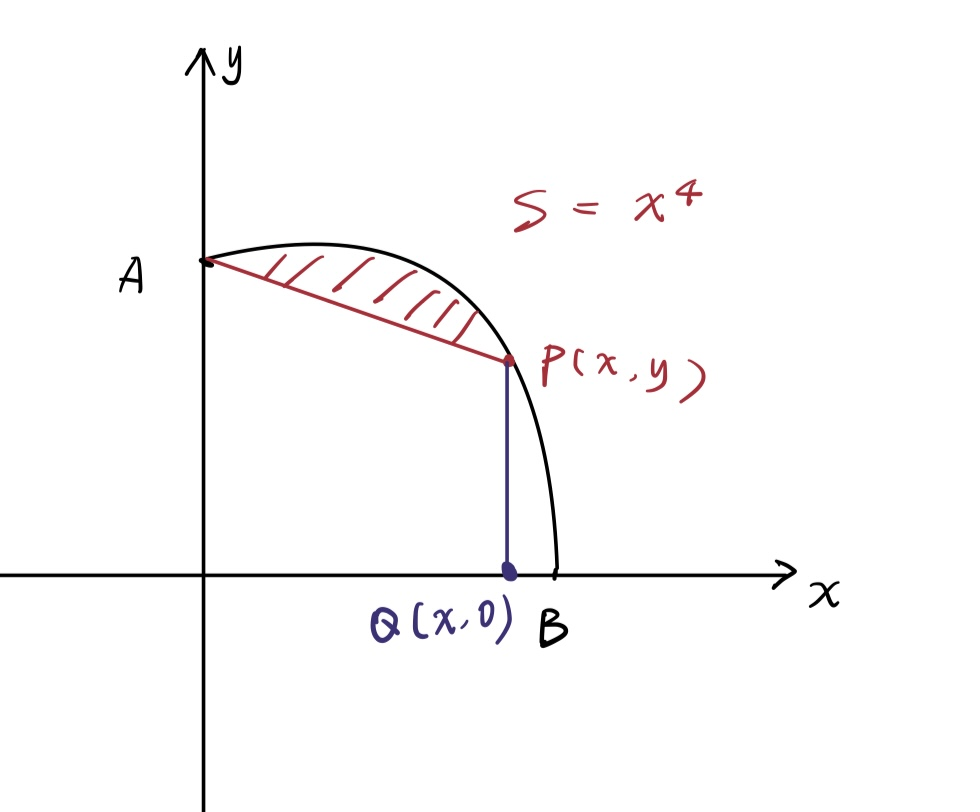
\includegraphics[width=15cm,height=10cm]{"figure/Summary/平面示意图.jpg"}
	\caption{平面示意图}
\end{figure} 
\myspace{1}
\begin{solution}
	
	如上图所示:  
	$$S=\int_{0}^{x}f(t)dt-\dfrac{1+f(x)}{2}x=x^4$$
	
	两边同时求导得到:  
	$$\dfrac{xf'(x)-f(x)}{x^2}=-\dfrac{8x^3+1}{x^2}\Rightarrow \dfrac{f(x)}{x}=-4x^2+\dfrac{1}{x}+C$$
	
	我们得到:  $f(x)=-4x^3+Cx+1$,又因为:  $\int_{0}^{1}f(x)dx=\dfrac{3}{2}\Rightarrow C=3$
	
	综上所述,$L$的方程为:  $f(x)=-4x^3+3x+1$
\end{solution}
\begin{anymark}[注]
	[题目来源]:  $660 \ P_{216}$
\end{anymark}
\myspace{1}

19.设函数$z=\sqrt{x^2+y^2}f(\dfrac{y}{x})$,且$f(u)$可导,若$x\dfrac{\partial z}{\partial x}+y\dfrac{\partial z}{\partial y}=\dfrac{2y^2}{\sqrt{x^2+y^2}}$,求$f(1)$,$f'(1)$.
\myspace{1}
\begin{solution}
	
	我们可以得到:  
	$$\left\lbrace
	\begin{array}{l}
		\dfrac{\partial z}{\partial x}=\dfrac{x}{\sqrt{x^2+y^2}}f(\frac{y}{x})-\dfrac{y\sqrt{x^2+y^2}}{x^2}f'(\frac{y}{x})\\
		\dfrac{\partial z}{\partial y}=\dfrac{y}{\sqrt{x^2+y^2}}f(\frac{y}{x})+\dfrac{\sqrt{x^2+y^2}}{x}f'(\frac{y}{x})
	\end{array}
	\right. \Rightarrow x\dfrac{\partial z}{\partial x}+y\dfrac{\partial z}{\partial y}=\sqrt{x^2+y^2}f(\frac{y}{x})=\dfrac{2y^2}{\sqrt{x^2+y^2}}$$
	
	我们得到:  
	$$f(\frac{y}{x})=\dfrac{2y^2}{x^2+y^2}\Rightarrow \left\lbrace
	\begin{array}{l}
		f(x)=\dfrac{2x^2}{1+x^2}\\
		\\
		f'(x)=\dfrac{4x}{(1+x^2)^2}
	\end{array}
	\right. $$
	
	我们得到:  $f(1)=1,f'(1)=1$
\end{solution}
\begin{anymark}[注]
	[题目来源]:  $660 \ P_{244}$
\end{anymark}
\myspace{1}

20. 设函数$f(x,y)$可微且$f[x+1,ln(1+x)]=(1+x)^3+xln(1+x)(x+1)^{ln(x+1)}$,$f(x^2,x-1)=x^4e^{x-1}+(x-1)(x^2-1)x^{2(x-1)}$,求$df(1,0)$.
\begin{solution}
	
	我们令:  $$\left\lbrace
	\begin{array}{l}
		g(x)=xln(1+x)(x+1)^{ln(x+1)}\\
		h(x)=(x-1)(x^2-1)x^{2(x-1)}
	\end{array}
	\right. $$
	
	我们得到:  $$\left\lbrace
	\begin{array}{l}
		f[x+1,ln(1+x)]=(1+x)^3+g(x)\\
		f(x^2,x-1)=x^4e^{x-1}+h(x)
	\end{array}
	\right. $$
	
	我们在两边同时对$x$求导:  
	$$\left\lbrace
	\begin{array}{l}
		f'_{1}[x+1,ln(1+x)]+f'_{2}[x+1,ln(1+x)]\dfrac{1}{x+1}=3(1+x)^2+g'(x)\\
		2xf'_{1}(x^2,x-1)+f'_{2}(x^2,x-1)=(4x^3+x^4)e^{x-1}+h'(x)
	\end{array}
	\right. $$
	
	我们得到:  
	$$\left\lbrace
	\begin{array}{l}
		f'_{1}(1,0)+f'_{2}(1,0)=3+g'(0)\\
		2f'_{1}(1,0)+f'_{2}(1,0)=5+h'(1)
	\end{array}
	\right. $$
	
	又因为:  $g'(0)=h'(0)=0$
	$$f'_{1}(1,0)=2,\ f'_{2}(1,0)=1\Rightarrow df(1,0)=2dx+dy$$
\end{solution}
\begin{anymark}[注]
	[题目来源]:  $660 \ P_{245}$
\end{anymark}
\myspace{1}

21.求二重积分$I=\int_{0}^{1}dy\int_{y}^{1}\sqrt{x^2+y^2}dx$
\myspace{1}
\begin{solution}
	
	原二重积分等价于:  
	\begin{eqnarray*}
		I&=&\int_{0}^{\frac{\pi}{4}}d\theta\int_{0}^{\frac{1}{\cos \theta}}r^2dr\\
		&=&\int_{0}^{\frac{\pi}{4}}\dfrac{1}{3\cos^3\theta}d\theta\\
		I_{1}&=&\int_{0}^{\frac{\pi}{4}}\dfrac{1}{\cos^3\theta}d\theta\\
		&=&\int_{0}^{\frac{\pi}{4}}\dfrac{1}{\cos\theta}d\tan \theta\\
		&=&\dfrac{tan \theta}{\cos\theta}|_{0}^{\frac{\pi}{4}}-\int_{0}^{\frac{\pi}{4}}\dfrac{1-\cos^2\theta}{\cos^3\theta}d\theta\\
		&=&\sqrt{2}-I_{1}+\int_{0}^{\frac{\pi}{4}}\dfrac{1}{\cos \theta}d\theta\\
		&=&\sqrt{2}+ln|\frac{1+\sin\theta}{\cos\theta}|_{0}^{\frac{\pi}{4}}-I_{1}\\
		&=&\sqrt{2}+ln(\sqrt{2}+1)-I_{1}\\
	I_{1}&=&\dfrac{\sqrt{2}+ln(\sqrt{2}+1)}{2}\Rightarrow I=\dfrac{\sqrt{2}+ln(\sqrt{2}+1)}{6}
	\end{eqnarray*}
\end{solution}
\begin{anymark}[注]
	[题目来源]:  $660 \ P_{269}$
\end{anymark}
\myspace{1}

22. 已知函数$f(x,y)$在点$(0,0)$某邻域内连续,且$\lim\limits_{(x,y)\rightarrow(0,0)}\dfrac{f(x,y)+4x^2-y^2}{x^4+x^2y^2+y^4}=1$.
\begin{itemize}
	\item \hl{A}. 点$(0,0)$不是$f(x,y)$的极值点
	\item B. 点$(0,0)$是$f(x,y)$的极大值点
	\item C. 点$(0,0)$是$f(x,y)$的极小值点
	\item D. 所给条件不足以判断点$(0,0)$是否为$f(x,y)$的极值点
\end{itemize}
\myspace{1}
\begin{solution}
	
	我们可以得到:  
	$$f(x,y)=y^2-4x^2+(x^4+x^2y^2+y^4)(1+\alpha),\ \lim\limits_{(x,y)\rightarrow(0,0)}\alpha(x,y)=0$$
	$$f(0,0)=\lim\limits_{(x,y)\rightarrow(0,0)}f(x,y)=0$$
	
	我们有:  $$\left\lbrace
	\begin{array}{l}
		f(0,y)=y^2+y^4(1+\alpha)\\
		f(x,0)=-4x^2+x^4(1+\alpha)
	\end{array}
	\right. $$
	
	我们有:  $$\left\lbrace
	\begin{array}{l}
		x\rightarrow 0, f(x,0)<f(0,0)\\
		y\rightarrow 0, f(0,y)>f(0,0)
	\end{array}
	\right. $$
	
	在$(0,0)$的邻域内,存在比$f(0,0)$大的函数值,也存在比$f(0,0)$小的函数值
	
	综上所述,$f(0,0)$不是极值点.
\end{solution}
\begin{anymark}[注]
	[题目来源]:  $660 \ P_{254}$
\end{anymark}
\myspace{1}

23. 求$(x+2)y''+x(y')^2=y'$的通解.
\myspace{1}
\begin{solution}
	
	我们不妨设$y'(x)=p$,我们有:  $y''=\frac{dp}{dx}$,原方程等价于:  
	$$(x+2)\frac{dp}{dx}+xp^2=p\Rightarrow \frac{dp}{dx}-\frac{p}{x+2}=-\dfrac{x}{x+2}p^2$$
	
	我们两边同时除以$-p^2$得到:  
	$$\frac{dp}{dx}(-\frac{1}{p^2})+\dfrac{1}{x+2}\frac{1}{p}=\frac{x}{x+2}\Rightarrow \frac{dp^{-1}}{dx}+\frac{p^{-1}}{x+2}=\frac{x}{x+2}$$
	
	我们可以得到:  $p^{-1}=\frac{1}{x+2}(\int xdx+C)=\frac{x^2+C_{1}}{2x+4}$
	
	我们有:  $\dfrac{dy}{dx}=\dfrac{2x+4}{x^2+C_{1}}$
	
	(1). 当$C_{1}>0$时,$y=ln(x^2+C_{1})+\dfrac{4}{\sqrt{C_{1}}}\arctan \dfrac{x}{\sqrt{C_{1}}}+C_{2}$
	
	(2). 当$C_{1}=0$时,$y=2ln|x|-\dfrac{4}{x}+C_{2}$
	
	(3). 当$C_{1}<0$时,$y=ln|x^2+C_{1}|+\dfrac{2}{\sqrt{-C_{1}}}ln|\dfrac{x-\sqrt{-C_{1}}}{x+\sqrt{-C_{1}}}|+C_{2}$
\end{solution}
\myspace{1}

24. 设函数$f(t)$在$[0,+\infty)$上连续,且满足方程$f(t)=e^{4\pi t^2}+\iint\limits_{x^2+y^2\leq 4t^2}f(\frac{1}{2}\sqrt{x^2+y^2})dxdy$,求$f(t)$.
\myspace{1}
\begin{solution}
	
	原方程可以化为:  
	\begin{eqnarray*}
		f(t)&=&e^{4\pi t^2}+\int_{0}^{2\pi}d\theta\int_{0}^{2t}rf(\frac{1}{2}r)dr\\
		&=&e^{4\pi t^2}+2\pi\int_{0}^{2t}rf(\frac{1}{2}r)dr
	\end{eqnarray*}
	
	我们对等式两边对$t$求导得到:  
	$$f'(t)=8\pi te^{4\pi t^2}+8\pi tf(t)\Rightarrow f'(t)-8\pi tf(t)=8\pi te^{4\pi t^2}$$
	
	我们有:  
	$$f(t)=(\int 8\pi te^{4\pi t^2}e^{\int-8\pi t}dt+C)e^{\int8\pi t}=( 4\pi t^2+C)e^{4\pi t^2}$$
	
	因为$f(0)=1\Rightarrow C=1$
	
	综上所述,$f(t)=( 4\pi t^2+1)e^{4\pi t^2}$
\end{solution}
\myspace{1}

25. 证明:  $r(A)=r(A^{T})=r(AA^{T})=r(A^{T}A)\Leftrightarrow$方程组$Ax=O$与方程组$A^{T}Ax=0$同解.
\myspace{1}
\begin{solution}
	
	(1). $Ax=0$的任意一个解$\alpha$满足:  $A\alpha=0$
	
	我们得到:  $A^{T}(A\alpha)=A^{T}0=0$,说明$Ax=0$的解都是$A^{T}Ax=0$的解.
	
	(2). $A^{T}Ax=0\Rightarrow x^{T}A^{T}Ax=0\Rightarrow (Ax)^{T}(Ax)=0$
	
	$Ax$是一个列向量,$(Ax)^{T}(Ax)=|Ax|\geq 0\Rightarrow Ax=0$,说明$A^{T}Ax=0$的解都是$Ax=0$的解.
\end{solution}
\myspace{1}

26. 证明:  $n$阶矩阵$\left[ \begin{matrix}
	1&1&\cdots&1\\
	1&1&\cdots&1\\
	\vdots&\vdots& &\vdots\\
	1&1&\cdots&1
\end{matrix}\right] $与$\left[ \begin{matrix}
0&\cdots&0&1\\
0&\cdots&0&2\\
\vdots&\vdots& &\vdots\\
0&\cdots&0&n
\end{matrix}\right] $相似.
\myspace{1}
\begin{solution}
	
	我们转化为证明矩阵$A,B$都相似于同一个对角矩阵.
	
	(1).$|\lambda E-A|=\left|  \begin{matrix}
		\lambda-1&-1&\cdots&-1\\
		-1&\lambda-1&\cdots&-1\\
		\vdots&\vdots& &\vdots\\
		-1&-1&\cdots&\lambda-1
	\end{matrix}\right|=(\lambda-n)\lambda^{n-1}$
	
	$A$为实对称矩阵,可以相似对角化为$\varLambda=\left[ \begin{matrix}
		n& & & \\
		 &0& & \\
		 & &\ddots&\\
		 & & & 0
	\end{matrix}\right] $.

	(2).$|\lambda E-A|=\left|  \begin{matrix}
		\lambda&0&\cdots&-1\\
		0&\lambda-1&\cdots&-2\\
		\vdots&\vdots& &\vdots\\
		0&0&\cdots&\lambda-n
	\end{matrix}\right|=(\lambda-n)\lambda^{n-1}$
	
	$B$有特征值$0,0,\cdots,n$,特征值$0$对应的特征向量有$num=n-rank(A)=n-1$个.
	
	$B$可以相似对角化为$\varLambda=\left[ \begin{matrix}
		n& & & \\
		&0& & \\
		& &\ddots&\\
		& & & 0
	\end{matrix}\right] $.

	我们由$A\sim \varLambda,\ B\sim \varLambda\Rightarrow A\sim B$
\end{solution}
\myspace{1}

27. 设$A=\left[ \begin{matrix}
	1&-2&0&0\\
	-1&0&0&0\\
	0&0&2&1\\
	0&0&0&2
\end{matrix}\right] $,求$A^n(n\geq 2)$
\myspace{1}
\begin{solution}
	
	我们设$B=\left[ \begin{matrix}
		1&-2\\-1&0
	\end{matrix}\right] ,\ C=\left[ \begin{matrix}
	2&1\\0&2
\end{matrix}\right]$,我们得到:  
$$A=\left[ \begin{matrix}
	B&0\\0&C
\end{matrix}\right]\Rightarrow A^{n}=\left[ \begin{matrix}
B^n&0\\0&C^n
\end{matrix}\right]$$

(1). $B^{n}$我们利用对角矩阵来求,我们将$B$对角化

$$|\lambda E-B|=|\begin{matrix}
	\lambda-1&2\\
	1&\lambda
\end{matrix}|=(\lambda-2)(\lambda+1)$$

当$\lambda=-1$时,$(-E-A)x=0\Rightarrow \left[\begin{matrix}
	-2&2\\1&-1
\end{matrix} \right]\left[\begin{matrix}
x_{1}\\x_{2}
\end{matrix} \right]=0$,我们取$\xi_{1}=(1,1)^T$

当$\lambda=2$时,$(2E-A)x=0\Rightarrow \left[\begin{matrix}
	1&2\\1&2
\end{matrix} \right]\left[\begin{matrix}
x_{1}\\x_{2}
\end{matrix} \right]=0$,我们取$\xi_{2}=(2,-1)^T$

我们取$P=[\xi_{1},\xi_{2}]$,\ $s.t. P^{-1}BP=\varLambda=\left[\begin{matrix}
	-1&\\ &2
\end{matrix} \right]$

我们得到:  $$B^n=P\varLambda^n P^{-1}=\left[\begin{matrix}
	1&2\\1&-1
\end{matrix} \right]\left[\begin{matrix}
(-1)^n&\\ &2^n
\end{matrix} \right]\left[\begin{matrix}
\dfrac{1}{3}&\dfrac{2}{3}\\\dfrac{1}{3}&-\dfrac{1}{3}
\end{matrix} \right]=\left[\begin{matrix}
\dfrac{(-1)^n+2^{n+1}}{3}&\dfrac{(-1)^n2-2^{n+1}}{3}\\
\\\dfrac{(-1)^n-2^n}{3}&\dfrac{(-1)^n2+2^n}{3}
\end{matrix} \right]$$

(2). $C^n=(2E+D)^n,\ D=\left[ \begin{matrix}
	0&1\\0&0
\end{matrix}\right],D^{n}=0(n\geq 2)$
$$C^n=C_{n}^{0}(2E)^n+C_{n}^{1}(2E)^{n-1}D+C_{n}^{2}(2E)^{n-2}D^2+\cdots=2^nE+n2^{n-1}D$$

我们得到:  $C^n=\left[ \begin{matrix}
	2^n&n2^{n-1}\\0&2^n
\end{matrix}\right]$

我们得到:  
$$A^n=\left[ \begin{matrix}
	B^n&0\\0&C^n
\end{matrix}\right]=\left[ \begin{matrix}
\dfrac{(-1)^n+2^{n+1}}{3}&\dfrac{(-1)^n2-2^{n+1}}{3}&0&0\\
\dfrac{(-1)^n-2^n}{3}&\dfrac{(-1)^n2+2^n}{3}&0&0\\
0&0&2^n&n2^{n-1}\\0&0&0&2^n
\end{matrix}\right]$$
\end{solution}
\myspace{1}

28. 已知$A$是三阶矩阵且$(A-E)^{-1}=A^2+A+E$,求$|A|$
\myspace{1}
\begin{solution}
	
	我们可以得到:  
	$$(A-E)(A-E)^{-1}=(A-E)(A^2+A+E)=E\Rightarrow A^3-E^3=E\Rightarrow A^3=2E$$
	
	我们可以得到:  $|A^3|=|A|^3=|2E|=2^3|E|=8\Rightarrow |A|=2$
\end{solution}
\begin{anymark}[注]
	[题目来源]:  $660 \ P_{349}$
\end{anymark}
\myspace{1}

29. 求$\int_{0}^{+\infty}e^{-2x}|\sin x|dx$
\myspace{1}
\begin{solution}
	
	方法一:  (积分变换)
	
	原积分可以化为:  
	\begin{eqnarray*}
		I&=&\int_{0}^{\pi}e^{-2x}\sin xdx+\int_{\pi}^{+\infty}e^{-2x}|\sin x|dx\\
		&=&\int_{0}^{\pi}e^{-2x}\sin xdx+e^{-2\pi}\int_{0}^{+\infty}e^{-2x}|\sin x|dx\\
		&=&\int_{0}^{\pi}e^{-2x}\sin xdx+e^{-2\pi}I
	\end{eqnarray*}

	我们得到:  
	$$I=\dfrac{\int_{0}^{\pi}e^{-2x}\sin xdx}{1-e^{-2\pi}}$$
	$$\int_{0}^{\pi}e^{-2x}\sin xdx=\dfrac{\left|\begin{matrix}
			-2e^{-2x}&\cos x\\e^{-2x}&\sin x \end{matrix}\right| }{5}|_{x=0}^{x=\pi}=\dfrac{1+e^{-2\pi}}{5}$$
	
	综上所述,我们得到:  $I=\dfrac{1+e^{-2\pi}}{5(1-e^{-2\pi})}$
\end{solution}
\begin{anymark}[思考]
	$$f(x)=e^{-ax}|\sin bx|,(a>0,b>0),\ \text{求}\int_{0}^{+\infty}f(x)dx$$
\begin{figure}[H]
	\centering
	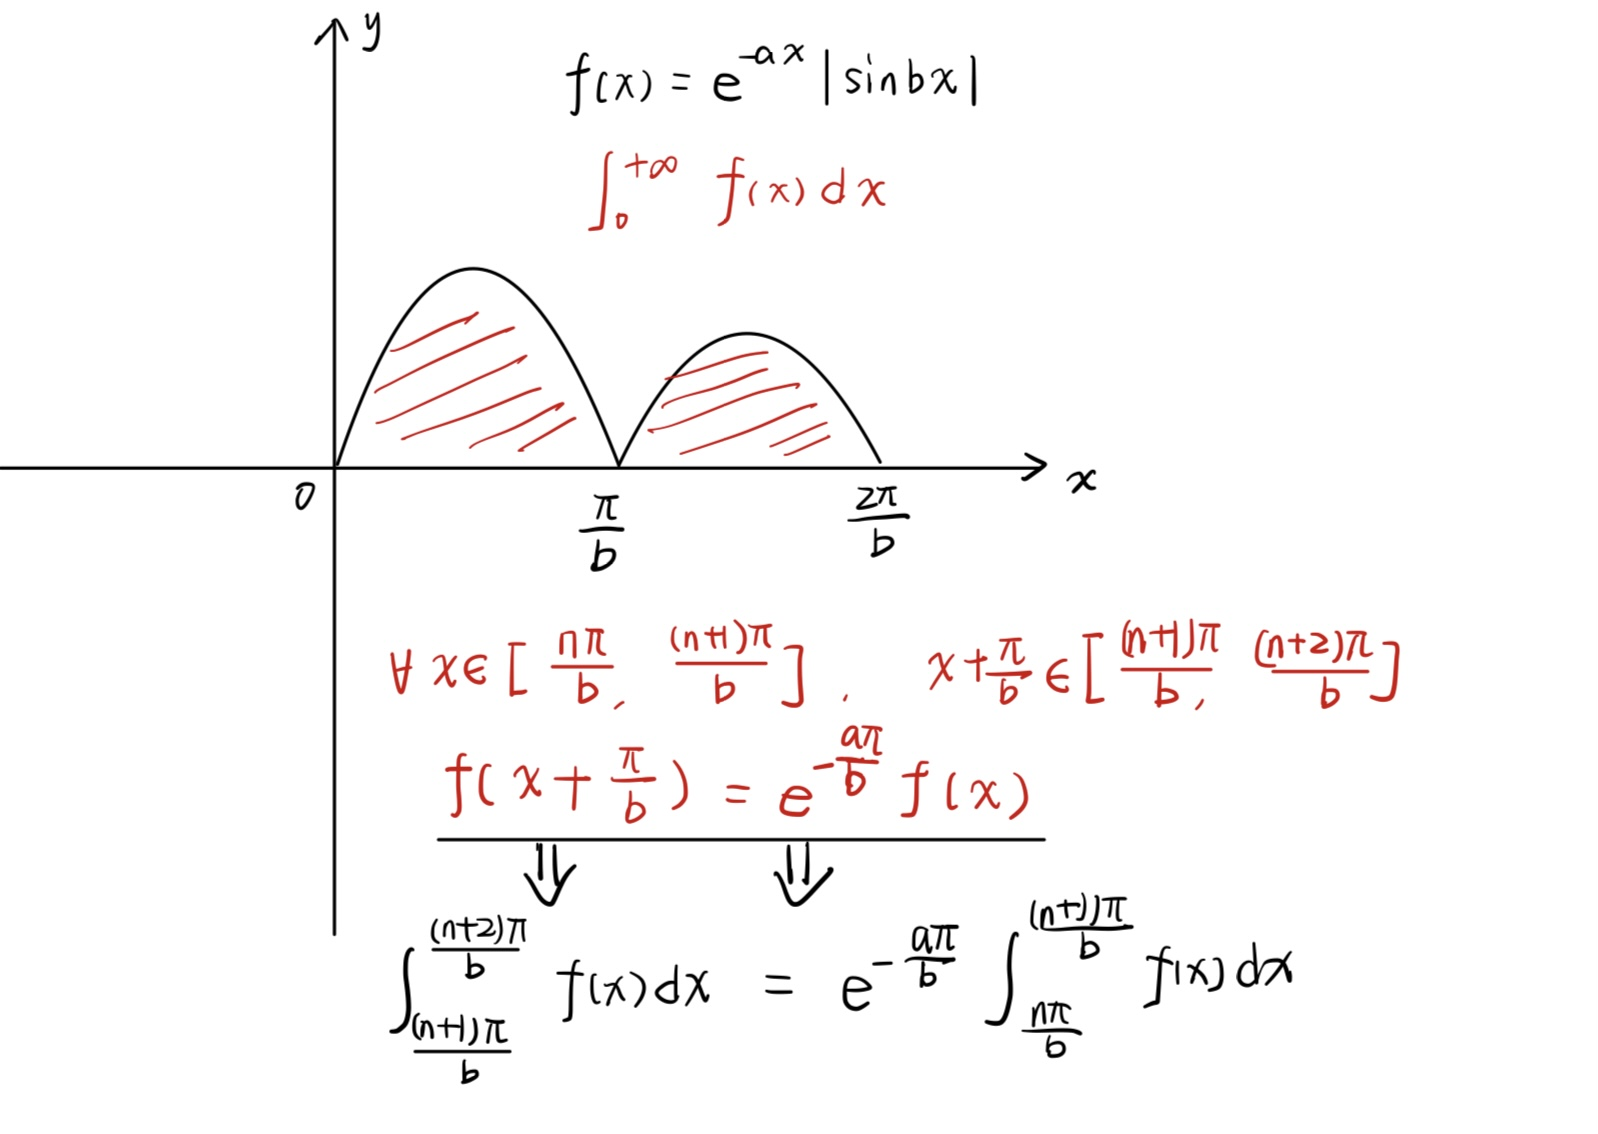
\includegraphics[width=15cm,height=10cm]{"figure/Summary/伪周期问题.jpg"}
	\caption{简易函数图示}
\end{figure} 	
	我们有:  
	$$\forall x\in[\dfrac{n\pi}{n},\dfrac{(n+1)\pi}{b}], f(x+\dfrac{\pi}{b})=e^{-\dfrac{a\pi}{b}}f(x)$$
	$$\int_{\dfrac{n\pi}{b}}^{\dfrac{(n+1)\pi}{b}}f(x)dx=e^{-\dfrac{a\pi}{b}}\int_{\dfrac{(n+1)\pi}{b}}^{\dfrac{(n+2)\pi}{b}}f(x)dx$$
	
	我们不妨设$A=\int_{0}^{\dfrac{\pi}{b}}f(x)dx,\ q=e^{-\dfrac{a\pi}{b}}$,我们有:  
	\begin{eqnarray*}
		\int_{0}^{+\infty}f(x)dx&=&\int_{0}^{\dfrac{\pi}{b}}f(x)dx+\int_{\dfrac{\pi}{b}}^{\dfrac{2\pi}{b}}f(x)dx+\cdots+int_{\dfrac{(n-1)\pi}{b}}^{\dfrac{n\pi}{b}}f(x)dx+\cdots\\
		&=&A+Aq+Aq^2+\cdots+Aq^{n}+\cdots\\
		&=&\lim\limits_{n\rightarrow+\infty}\dfrac{A(1-q^n)}{1-q}\\
		&=&\dfrac{A}{1-q}
	\end{eqnarray*}

	$$A=\int_{0}^{\dfrac{\pi}{b}}f(x)dx=G(\dfrac{\pi}{b})-G(0)$$
	$$G(x)=\dfrac{\left| \begin{matrix}
			(e^{-a})'&(\sin(bx))'\\e^{-a}&\sin(bx)
		\end{matrix}\right| }{a^2+b^2}\Rightarrow G(\dfrac{\pi}{b})-G(0)=\dfrac{b(1+e^{e^{-\dfrac{a\pi}{b}}})}{a^2+b^2}$$
	
	综上所述,我们得到:  
	$$\int_{0}^{+\infty}f(x)dx=\dfrac{b(1+e^{-\dfrac{a\pi}{b}})}{(a^2+b^2)(1-e^{-\dfrac{a\pi}{b}})}$$
\end{anymark}
\myspace{1}

30. 求$\int e^{ax}\sin bxdx$
\myspace{1}
\begin{solution}
	
	利用分部积分法,原不定积分可化为:  
	\begin{eqnarray*}
		I&=&\dfrac{1}{a}\int \sin (bx)d(e^{ax})\\
		&=&\dfrac{e^{ax}\sin (bx)}{a}-\dfrac{b}{a}\int e^{ax}\cos(bx)dx\\
		&=&\dfrac{e^{ax}\sin (bx)}{a}-\dfrac{b}{a^2}[e^{ax}\cos (bx)+b\int e^{ax}\sin (bx)dx]\\
		&=&\dfrac{e^{ax}\sin (bx)}{a}-\dfrac{b}{a^2}e^{ax}\cos (bx)-\dfrac{b^2}{a^2}I+C
	\end{eqnarray*}
	
	$$I=\dfrac{ae^{ax}\sin (bx)-be^{ax}\cos (bx)}{a^2+b^2}=\dfrac{\left|\begin{matrix}
			(e^{ax})' & e^{ax}\\(\sin (bx))' & \sin(bx)
		\end{matrix} \right|}{a^2+b^2}+C$$
	
	同样我们也可以得到:  
	$$\int e^{ax}\cos (bx)dx=\dfrac{\left|\begin{matrix}
			(e^{ax})' & e^{ax}\\(\cos (bx))' & \cos(bx)
		\end{matrix} \right|}{a^2+b^2}+C$$
\end{solution}
\myspace{1}

31. 设$x_{1}=a\geq 0$,$y_{1}=b\geq 0$,$a\leq b$,$x_{n+1}=\sqrt{x_{n}y_{n}},y_{n+1}=\dfrac{x_{n}+y_{n}}{2},(n=1,2,\cdots)$,证明:  $\lim\limits_{n\rightarrow +\infty}x_{n}=\lim\limits_{n\rightarrow +\infty}y_{n}$
\myspace{1}
\begin{solution}
	
	我们由:  $x_{1}=a\geq 0$,$y_{1}=b\geq 0$,$x_{n+1}=\sqrt{x_{n}y_{n}},y_{n+1}=\dfrac{x_{n}+y_{n}}{2}$,由归纳法可知:  
	$$x_{n}\geq 0, y_{n}\geq 0$$
	
	由基本不等式:  
	$$\dfrac{x_{n}+y_{n}}{2}\geq \sqrt{x_{n}y_{n}}\Rightarrow y_{n+1}\geq x_{n+1}$$
	
	又因为:  $x_{n+1}=\sqrt{x_{n}y_{n}}\geq x_{n}, y_{n+1}=\dfrac{x_{n}+y_{n}}{2}\leq y_{n}$.
	
	$x_{n}$单调递增,$y_{n}$单调递减,$x_{1}\leq x_{n}\leq y_{n}\leq y_{1}$
	
	$x_{n},y_{n}$单调且有界,数列$\{x_{n}\},\{y_{n}\}$均有极限,我们不妨设:  
	$$\left\lbrace
	\begin{array}{l}
		\lim\limits_{n\rightarrow +\infty}x_{n}=a\\
		\lim\limits_{n\rightarrow +\infty}y_{n}=b
	\end{array}
	\right. \Rightarrow \left\lbrace
	\begin{array}{l}
		a=\sqrt{ab}\\
		b=\dfrac{a+b}{2}
	\end{array}
	\right. \Rightarrow a=b$$
	
	综上所述,我们得到:  $\lim\limits_{n\rightarrow +\infty}x_{n}=\lim\limits_{n\rightarrow +\infty}y_{n}$
\end{solution}
\begin{anymark}[注]
	[题目来源]:  $880 \text{第一章基础}\ P_{11}$
\end{anymark}
\myspace{1}

32.设数列$\{a_{n}\}$满足$\lim\limits_{n\rightarrow+\infty}\dfrac{a_{n+1}}{a_{n}}=q$,且$|q|<1$,证明:  $\lim\limits_{n\rightarrow+\infty}a_{n}=0$
\myspace{1}
\begin{solution}
	
	我们考虑数列$\{|a_{n}|\}$,我们可以得到:  
	$$\lim\limits_{n\rightarrow +\infty}\dfrac{|a_{n+1}|}{|a_{n}|}=|q|\Rightarrow \exists\ M>0,\ n>M\text{时}, \dfrac{|a_{n+1}|}{|a_{n}|}<1$$
	
	又因为$|a_{n}|\geq 0$,我们可以知道$\{|a_{n}|\}$极限必定存在,我们不妨假设$\lim\limits_{n\rightarrow+\infty}|a_{n}|=a$.
	
	假设$a\neq 0$,我们可以得到:  $$\lim\limits_{n\rightarrow  +\infty}\dfrac{|a_{n+1}|}{|a_{n}|}=\dfrac{\lim\limits_{n\rightarrow  +\infty}|a_{n+1}|}{\lim\limits_{n\rightarrow  +\infty}|a_{n}|}=1$$
	
	这和$|q|<1$矛盾!!!
	
	
	综上所述,我们可以得到:  $\lim\limits_{n\rightarrow+\infty}a_{n}=0$
\end{solution}
\begin{anymark}[注]
	[题目来源]:  $880\text{第一章综合} \ P_{1}$
\end{anymark}
\myspace{1}

33. 设$x_{1}=1,x_{2}=2,x_{n+2}=\dfrac{1}{2}(x_{n}+x_{n+1})$,求$\lim\limits_{n\rightarrow+\infty}x_{n}$
\myspace{1}
\begin{solution}
	
	我们有:  $x_{n+1}-x_{n}=-\dfrac{1}{2}(x_{n}-x_{n-1})$
	
	我们得到:  数列$\{x_{n+1}-x_{n}\}$是以$1$为首项,$-\dfrac{1}{2}$为公比的等比数列.
	
	$$\sum\limits_{k=1}^{n}(x_{k+1}-x_{k})=x_{n+1}-x_{1}=\dfrac{1-(-(\dfrac{-1}{2})^{n}}{1+\dfrac{1}{2}}$$
	
	$$\lim\limits_{n\rightarrow +\infty}x_{n+1}=1+\dfrac{2}{3}=\dfrac{5}{3}$$
\end{solution}
\begin{anymark}[注]
	[题目来源]:  $880\text{第一章综合} \ P_{5}$
\end{anymark}
\myspace{1}

34. 设$f_{n}(x)=1-(1-\cos x)^n(n=1,2,\cdots)$

(1). 证明:  方程$f_{n}(x)=\dfrac{1}{2}$在$(0,\dfrac{\pi}{2})$内有且只有一个实数根$x_{n}$

(2). 设$x_{n}\in(0,\dfrac{\pi}{2})$,满足$f_{n}(x)=\dfrac{1}{2}$,证明:  $$\arccos \dfrac{1}{n}<x_{n}<\dfrac{\pi}{2},\text{且}\lim\limits_{n\rightarrow +\infty}x_{n}=\dfrac{\pi}{2}$$
\myspace{1}
\begin{solution}
	
	我们构造辅助函数:  $G_{n}(x)=\dfrac{1}{2}-(1-\cos x)^{n}$
	
	(1). $$G_{n}'(x)=-n\sin x(1-\cos x)^{n-1}$$
	
	当$x\in(0,\dfrac{\pi}{2})$,$G_{n}'(x)<0$,$\ G_{n}(x)$在$(0,\dfrac{\pi}{2})$单调递减.
	
	$$G_{n}(0)=\dfrac{1}{2}>0,\ G_{n}(\dfrac{\pi}{2})=-\dfrac{\pi}{2}<0$$
	
	我们根据零点定理,可以得到:  $\exists \text{唯一的}x_{n}\in(0,\dfrac{\pi}{2}),\ s.t. G_{n}(x_{n})=0$
	
	(2). 我们将$x=\arccos\dfrac{1}{n}$代入$G_{n}(x)$得到:  
	$$G_{n}(\arccos\dfrac{1}{n})=\dfrac{1}{2}-(1-\dfrac{1}{n})^{n}$$
	
	我们知道:  $\lim\limits_{n\rightarrow+\infty}(1-\dfrac{1}{n})^{n}=\dfrac{1}{e}\Rightarrow G_{n}(\arccos\dfrac{1}{n})>0$
	
	我们需要证明:  $(1-\dfrac{1}{n})^n$单调性,我们构造辅助函数:  $H(x)=e^{xln(1-\dfrac{1}{x})},x\geq 2$
	
	我们可以得到:  $H'(x)=e^{xln(1-\dfrac{1}{x})}[ln(1-\dfrac{1}{x})+\dfrac{1}{x-1}]>0$,$H(x)$单调递增.
	
	所以$G_{n}(\arccos\dfrac{1}{n})$单调递减,且$\lim\limits_{n\rightarrow+\infty}G_{n}(\arccos\dfrac{1}{n})=\dfrac{1}{2}-\dfrac{1}{e}>0$,我们得到:  $$\arccos \dfrac{1}{n}<x_{n}<\dfrac{\pi}{2}$$
	
	我们再由夹逼定理可以得到:  
	$$\left\lbrace
	\begin{array}{l}
		\lim\limits_{n\rightarrow  +\infty}\arccos \dfrac{1}{n}=\dfrac{\pi}{2}\\
		\lim\limits_{n\rightarrow  +\infty}\dfrac{\pi}{2}=\dfrac{\pi}{2}
	\end{array}
	\right. \Rightarrow \lim\limits_{n\rightarrow +\infty}x_{n}=\dfrac{\pi}{2}$$
	
\end{solution}
\begin{anymark}[注]
	[题目来源]:  $880\text{第一章综合} \ P_{6}$
\end{anymark}
\myspace{1}

35. 设$x_{1}>0$,数列$\{x_{n}\}$满足$x_{n+1}=ln(e^{x_{n}}-1)-ln x_{n}$,证明:  $\lim\limits_{n\rightarrow +\infty}x_{n}$存在并求其值.
\myspace{1}
\begin{solution}
	
	我们由:  $x_{n+1}=ln(e^{x_{n}}-1)-ln x_{n}$可以得到:  
	$$e^{x_{n+1}}=\dfrac{e^{x_{n}}-1}{x_{n}}$$
	
	我们构造辅助函数$f(x)=e^x-x-1$,$f'(x)=e^{x}-1$
	
	当$x>0$时,我们知道:  $f'(x)>0$,$f(x)$单调递增,$f(x)>f(0)=0\Rightarrow  x>0,\dfrac{e^x-1}{x}>1$
	
	我们有$x_{1}>0\Rightarrow e^{x_{2}}>1\Rightarrow x_{2}>0$,我们由归纳法可知:  $x_{n}>0$,数列$\{ x_{n}\}$有下界.
	
	我们由拉格朗日中值定理可以得到:  
	$$e^{x_{n+1}}=\dfrac{e^{x_{n}}-1}{x_{n}}=e^{\xi},\text{其中}\xi\in(0,x_{n})$$
	
	我们得到:  $x_{n+1}=\xi<x_{n}$,数列$\{x_{n}\}$单调递减,我们由单调有界准则可以得到:  数列$\{x_{n}\}$极限必定存在,我们不妨假设$\lim\limits_{n\rightarrow +\infty}x_{n}=a$,我们有:  
	$$e^{a}=\dfrac{e^a-1}{a}\Rightarrow a=0$$
	
	综上所述,数列$\{x_{n}\}$极限存在,其值为$0$
\end{solution}
\begin{anymark}[注]
	[题目来源]:  $880\text{第一章综合} \ P_{13}$
\end{anymark}
\myspace{1}

36. 设$f(x)$在$(a,b)$内连续,且$\lim\limits_{x\rightarrow a^{+}}f(x)=\lim\limits_{x\rightarrow b^{-}}f(x)=-\infty$,证明:  $f(x)$在$(a,b)$内有最大值.
\myspace{1}
\begin{solution}
	
	我们不妨取$M=f(\dfrac{a+b}{2})$,我们有$\lim\limits_{x\rightarrow a^{+}}f(x)=\lim\limits_{x\rightarrow b^{-}}f(x)=-\infty$
	
	我们由极限定义可以得到:  
	$$\left\lbrace
	\begin{array}{l}
		\exists a<c<\dfrac{a+b}{2},\ x\in(a,c),\ s.t. f(x)\leq f(\dfrac{a+b}{2})\\
		\exists \dfrac{a+b}{2}<d<b,\ x\in(d,b),\ s.t. f(x)\leq f(\dfrac{a+b}{2})
	\end{array}
	\right. $$
	
	在闭区间$[c,d]$上,$f(x)$连续,$f(x)$必定有最大值为$f(\xi),\ \xi\in[c,d]$,且$f(\xi)\geq f(\dfrac{a+b}{2})$.在区间$(a,c)\cup (d,b)$上,我们有$f(x)\leq f(\dfrac{a+b}{2})$.
	
	综上所述,$f(x)$在区间$(a,b)$内有最大值.
\end{solution}
\begin{anymark}[注]
	[题目来源]:  $880\text{第一章综合} \ P_{16}$
\end{anymark}
\myspace{1}

37. 设$f(x)$在$[a,b]$上可导,且$|f'(x)|<1$,当$x\in[a,b]$时,有$a<f(x)<b$,$F(x)=\dfrac{x+f(x)}{2}$,证明:  

(1). $\exists x^{*}\in(a,b),\ s.t. F(x^{*})=x^{*}$

(2). 对$x_{0}\in[a,b]$,数列$\{x_{n}\}$满足$x_{n+1}=F(x_{n}),(n=0,1,2,\cdots)$,有$\lim\limits_{n\rightarrow+\infty}x_{n}=x^{*}$
\myspace{1}
\begin{solution}
	
	(1). 我们构造辅助函数:  $G(x)=F(x)-x=\dfrac{f(x)-x}{2}$,我们有:  $G'(x)=\dfrac{f'(x)-1}{2}$
	
	又因为:  $|f'(x)|<1\Rightarrow G'(x)<0\Rightarrow G(x)\text{单调递减}$
	$$\left\lbrace
	\begin{array}{l}
		G(a)=\dfrac{f(a)-a}{2}>0\\
		G(b)=\dfrac{f(b)-b}{2}<0
	\end{array}
	\right. \Rightarrow G(a)G(b)<0$$
	
	我们根据零点定理可知:  $\exists x^{*}\in(a,b),\ s.t. G(x^{*})=0\Rightarrow \exists x^{*}\in(a,b),\ s.t. F(x^{*})=x^{*}$
	
	(2). 
	$F'(x)=\dfrac{1+f'(x)}{2}\geq 0\Rightarrow F(x)\text{单调递增}$
	
	(i). 当$x_{0}=x^{*}$时,$x_{n}=x^{*}$,此时$\lim\limits_{n\rightarrow +\infty}x_{n}=x^{*}$
	
	(ii). 当$x_{0}>x^{*}$时,我们有$G(x^{*})>G(x_{0})\Rightarrow F(x_{0})<x_{0}\Rightarrow x_{1}<x_{0}$
	
	当$n=1$时,$x_{1}<x_{0}$;
	
	当$n=k$时,$x_{k}<x_{k-1}$成立,当$n=k+1$时,我们有$F(x_{k})<F(x_{k-1})\Rightarrow x_{k+1}<x_{k}$
	
	我们得到数列$\{x_{n}\}$单调递减,且$x_{0}\in[a,b],\ x_{n}=\dfrac{x_{n}+f(x_{n})}{2},\ a<f(x)<b\Rightarrow x_{n}\in[a,b]$,数列$\{x_{n}\}$单调递减且有下界,极限必定存在.
	
	我们不妨假设数列$\{x_{n}\}$的极限为$A$,我们有:  $A=\dfrac{A+f(A)}{2}\Rightarrow F(A)=A\Rightarrow A=x^{*}$
	
	(iii). 当$x_{0}<x_{*}$时,我们有$G(x^{*})<G(x_{0})\Rightarrow F(x_{0})>x_{0}\Rightarrow x_{1}>x_{0}$
	
	当$n=1$时,$x_{1}>x_{0}$;
	
	当$n=k$时,$x_{k}>x_{k-1}$成立,当$n=k+1$时,我们有$F(x_{k})>F(x_{k-1})\Rightarrow x_{k+1}>x_{k}$
	
	我们得到数列$\{x_{n}\}$单调递增,且$x_{0}\in[a,b],\ x_{n}=\dfrac{x_{n}+f(x_{n})}{2},\ a<f(x)<b\Rightarrow x_{n}\in[a,b]$,数列$\{x_{n}\}$单调递增且有上界,极限必定存在.
	
	我们不妨假设数列$\{x_{n}\}$的极限为$A$,我们有:  $A=\dfrac{A+f(A)}{2}\Rightarrow F(A)=A\Rightarrow A=x^{*}$
	
	综上所述,我们得到:  $\lim\limits_{n\rightarrow+\infty}x_{n}=x^{*}$
\end{solution}
\begin{anymark}[注]
	[题目来源]:  $880\text{第一章扩展} \ P_{1}$
\end{anymark}
\myspace{1}

38. (1).设$f(x)$是$[0,+\infty)$上单调减少且非负的连续函数,证明:  $$f(k+1)\leq \int_{k}^{k+1}f(x)dx\leq f(k),\ k=1,2,\cdots$$

(2). 证明:  $ln(1+n)\leq 1+\dfrac{1}{2}+\cdots+\dfrac{1}{n}\leq 1+ln n$,求极限$\lim\limits_{n\rightarrow+\infty}\dfrac{1+\dfrac{1}{2}+\cdots+\dfrac{1}{n}}{ln n}$
\myspace{1}
\begin{solution}
	
	(1). 我们由$f(x)$单调减少且非负得到:  
	$$0\leq f(k+1)\leq f(x)\leq f(k),\ x\in[k,k+1]$$
	
	我们对上述不等式在$[k,k+1]$上同时求定积分得到:  
	$$\int_{k}^{k+1}f(k+1)dx\leq \int_{k}^{k+1}f(x)dx\leq \int_{k}^{k+1}f(k)dx\Rightarrow f(k+1)\leq \int_{k}^{k+1}f(x)dx\leq f(k)$$
	
	(2). 我们构造辅助函数$f(x)=\dfrac{1}{x}$,我们可以知道$f(x)$在$(0,+\infty)$上单调递减且非负,我们由(1)可以知道:  
	$$\left\lbrace
	\begin{array}{l}
		\dfrac{1}{2}\leq \int_{1}^{2}\dfrac{1}{x}dx\leq 1\\
		\dfrac{1}{3}\leq \int_{2}^{3}\dfrac{1}{x}dx\leq \dfrac{1}{2}\\
		\cdots\\
		\dfrac{1}{n}\leq \int_{n-1}^{n}\dfrac{1}{x}dx\leq \dfrac{1}{n-1}\\
		\dfrac{1}{n+1}\leq \int_{n}^{n+1}\dfrac{1}{x}dx\leq \dfrac{1}{n}
	\end{array}
	\right. \Rightarrow \left\lbrace
	\begin{array}{l}
		\sum\limits_{k=2}^{n+1}\dfrac{1}{k}\leq \int_{1}^{n+1}\dfrac{1}{x}=ln(1+n)\leq \sum\limits_{k=1}^{n}\dfrac{1}{k}\\
		\sum\limits_{k=2}^{n}\dfrac{1}{k}\leq \int_{1}^{n}\dfrac{1}{x}=ln n\\
		\sum\limits_{k=1}^{n}\dfrac{1}{k}=1+\sum\limits_{k=2}^{n}\dfrac{1}{k}\leq 1+ln n
	\end{array}
	\right. $$
	
	我们由夹逼定理可以得到:  
	$$\left\lbrace
	\begin{array}{l}
		\lim\limits_{n\rightarrow +\infty}\dfrac{ln(1+n)}{ln n}=1\\
		\lim\limits_{n\rightarrow +\infty}\dfrac{1+ln n}{ln n}=1
	\end{array}
	\right. \Rightarrow \lim\limits_{n\rightarrow  +\infty}\dfrac{1+\dfrac{1}{2}+\cdots+\dfrac{1}{n}}{ln n}=1$$
\end{solution}
\begin{anymark}[注]
	[题目来源]:  $880\text{第一章扩展} \ P_{2}$
\end{anymark}
\myspace{1}

39. 矩阵的谱分解定理
\begin{definition}[代数重复度]
	设$\lambda_{1},\lambda_{2},\cdots,\lambda_{k}$是矩阵$A\in \mathbb{C}^{n\times n}$的相异特征值,其重数分别为$r_{1},r_{2},\cdots,r_{k}$,称$r_{i}$为矩阵$A$的特征值$\lambda_{i}$的代数重复度.
\end{definition}
\begin{definition}[几何重复度]
	齐次方程组$Ax=\lambda_{i}x\ (i=1,2,\cdots,k)$的解空间$V_{\lambda_{i}}$称为$A$的对应于特征值$\lambda_{i}$的特征空间,则$V_{\lambda_{i}}$的维数称为$A$的特征值$\lambda_{i}$的几何重复度.
\end{definition}
\begin{definition}[单纯矩阵]
	若矩阵$A$的每一个特征值的代数重复度与几何重复度相等,则称矩阵$A$为单纯矩阵.
\end{definition}
\begin{definition}[幂等矩阵]
	若$A$为方阵,且$A^2=A$,则称$A$为幂等矩阵.
\end{definition}
\begin{property}[幂等矩阵$A$性质]
	\begin{itemize}
		\item (1). $A$是单纯矩阵,且其$Jordan$标准型为$\left(\begin{matrix}
			I_{r}&0\\0&0
		\end{matrix} \right) $
		\item (2). $A$的特征值只能为$0$或者$1$
		\item (3). $rank(A)=tr(A)$
		\item (4). $Ax=x\Leftrightarrow x\in\mathbb{R}(A)$
		\item (5). $A$一定可以相似对角化
	\end{itemize}
\end{property}
\begin{theorem}[谱分解定理]\label{the: 谱分解定理}
	设$A\in\mathbb{C}^{n\times n}$是单纯矩阵,矩阵$A$有$k$个相异特征值$\lambda_{i}\ (i=1,2,\cdots,k)$,$\exists A_{i}\in \mathbb{C}^{n\times n}\ (i=1,2,\cdots,k)$,使得
	$$A=\sum\limits_{i=1}^{k}\lambda_{i}G_{i}$$
	
	此式称为矩阵$A$的谱分解,$G_{1},G_{2},\cdots,G_{k}$称为$A$的族谱,且满足一下性质:  
	\begin{property}[谱分解谱族$G_{i}$性质]
		\begin{itemize}
			\item (1). 幂等性:  $G_{i}^2=G_{i}$
			\item (2). 分离性:  $G_{i}G_{j}=0\ (i\neq j)$
			\item (3). 可加性:  $\sum\limits_{i=1}^{k}G_{i}=E_{n}$
		\end{itemize}
	\end{property}
	\begin{corollary}[谱族$G_{i}$推论]
		\begin{itemize}
			\item $AG_{i}=G_{i}A=\lambda_{i}G_{i}$
			\item $rank(G_{i})=m_{i}$
			\item $G_{i}$是唯一的,$G$的族谱是唯一的.
		\end{itemize}
	\end{corollary}
	\begin{proposition}
		矩阵$A$是单纯矩阵等价为存在$k$个矩阵$G_{i},\ (i=1,2,\cdots,k)$满足:  
		\begin{itemize}
			\item (1). $G_{i}G_{j}=\left\lbrace
			\begin{array}{l}
				G_{i},\ i=j\\0,\ i\neq j
			\end{array}
			\right. $
			\item (2). $\sum\limits_{i=1}^{k}G_{i}=E_{n}$
			\item (3). $A=\sum\limits_{i=1}^{k}\lambda_{i}G_{i}$
			\item (4). $f(A)$为任意多项式,则$$f(A)=\sum\limits_{i=1}^{k}f(\lambda_{i})G_{i}$$
			\item (5). $A^m=\sum\limits_{i=1}^{k}\lambda_{i}^mG_{i}$
		\end{itemize}
	\end{proposition}
\end{theorem}
\begin{anymark}[证明]
	1. 必要性
	 
	(1). 当$k=n$时:  
	
	我们由$A$是单纯矩阵可以得到矩阵$A$可以相似对角化
	$$A=P\Lambda P^{-1},\text{其中}\Lambda=diag\{\lambda_{1},\lambda_{2},\cdots,\lambda_{n}\}$$
	
	我们不妨设$P=(v_{1},v_{2},\cdots,v_{n})$,$P^{-1}=\left( \begin{matrix}
		\omega_{1}^{T}\\\omega_{2}^{T}\\ \vdots\\\omega_{n}^{T}
	\end{matrix}\right) $,我们可以得到:  
	$$A=(v_{1},v_{2},\cdots,v_{n})\left[\begin{matrix}
		\lambda_{1}&0&\cdots&0\\
		0&\lambda_{2}&\cdots&0\\
		\cdots&\cdots&\cdots&\cdots\\
		0&0&\cdots&\lambda_{n}
	\end{matrix} \right] \left( \begin{matrix}
		\omega_{1}^{T}\\\omega_{2}^{T}\\ \vdots\\\omega_{n}^{T}
	\end{matrix}\right) \Rightarrow A=\sum\limits_{i=1}^{n}\lambda_{i}v_{i}\omega_{i}^{T}=\sum\limits_{i=1}^{n}\lambda_{i}G_{i},\ \text{其中}G_{i}=v_{i}\omega_{i}^{T}$$
	
	我们由$\left\lbrace
	\begin{array}{l}
		P^{-1}P=E_{n}\\
		PP^{-1}=E_{n}
	\end{array}
	\right.\Rightarrow\left\lbrace
	\begin{array}{l}
		\omega_{i}^{T}v_{j}=\left\lbrace
		\begin{array}{l}
			1,\ i=j\\
			0,\ i\neq j
		\end{array}
		\right. \\
		\sum\limits_{i=1}^{n}v_{i}\omega_{i}^{T}=\sum\limits_{i=1}^{n}G_{i}=E_{n}
	\end{array}
	\right.$
	
	对于任意$i,j\in(1,n),G_{i}G_{j}=v_{i}(\omega_{i}^{T}v_{j})\omega_{j}^{T}$,我们可以得到:  
	$$G_{i}G_{j}=\left\lbrace
	\begin{array}{l}
		v_{i}\omega_{i}^{T}=G_{i},\ i=j\\
		0,\ i\neq j
	\end{array}
	\right. \Rightarrow A_{i}\text{是幂等矩阵}$$
	
	(2). 当$k<n$时:  
	
	我们由矩阵$A$是单纯矩阵,可以得到:  $A=P\Lambda P^{-1}$
	$$\left\lbrace
	\begin{array}{l}
		P=(v_{11},v_{12},\cdots,v_{1r_{1}},v_{21},v_{22},\cdots,v_{2r_{2}},\cdots,v_{k1},v_{k2},\cdots,v_{kr_{k}})\\
		P^{-1}=(\omega_{11}^{T},\omega_{12}^{T},\cdots,\omega_{1r_{1}}^{T},\omega_{21}^{T},\omega_{22}^{T},\cdots,\omega_{2r_{2}}^{T},\cdots,\omega_{k1}^{T},\omega_{k2}^{T},\cdots,\omega_{kr_{k}}^{T})^{T}
	\end{array}
	\right. $$
	$$A=\sum\limits_{i=1}^{k}\lambda_{i}\sum\limits_{j=1}^{r_{i}}B_{ij}\stackrel{G_{i}=\sum\limits_{j=1}^{r_{i}}B_{ij}}{\longrightarrow}A=\sum\limits_{i=1}^{k}\lambda_{i}G_{i}$$
	$$P^{-1}P=E_{n}\Rightarrow \omega_{ij}^{T}v_{lk}=\left\lbrace
	\begin{array}{l}
		1,\ i=l,j=k\\
		0,\ i\neq l\text{或}j\neq k
	\end{array}
	\right. $$
	$$B_{ij}B_{lk}=v_{ij}(\omega_{ij}^{T}v_{lk})\omega_{lk}^{T}=\left\lbrace
	\begin{array}{l}
		B_{ij},\ i=l,j=k\\
		0,\ i\neq l\text{或}j\neq k
	\end{array}
	\right. \Rightarrow G_{i}G_{j}=\sum\limits_{p=1}^{r_{i}}B_{ip}\sum\limits_{q=1}^{r_{j}}B_{jq}=\left\lbrace
	\begin{array}{l}
		G_{i},\ i=j\\0,\ i\neq j
	\end{array}
	\right. $$
	$$\sum\limits_{i=1}^{k}G_{i}=\sum\limits_{i=1}^{n}B_{i}=E_{n}$$
	(2). 充分性
	
	我们首先可以得到矩阵$G_{i}$均为幂等矩阵,我们不妨设$dim\mathbb{R}(G_{i})=n_{i}$,我们可以得到:  
	$$n_{i}=tr(G_{i})\Rightarrow \sum\limits_{i=1}^{k}n_{i}=\sum\limits_{i=1}^{k}tr(G_{i})=tr(\sum\limits_{i=1}^{k}G_{i})=tr(E_{n})=n$$
	
	我们取$X_{i}$为$\mathbb{R}(G_{i})$的基列构成的阵,则$X=(X_{1},X_{2},\cdots,X_{k})$是$n\times n$矩阵,且$G_{i}$的列向量都可以由$X_{i}$线性表出,我们可以得到:  
	$$G_{i}=(X_{i}\beta_{1},X_{i}\beta_{2},\cdots,X_{i}\beta_{n})=X_{i}Y_{i}$$
	$$XY=(X_{1},X_{2},\cdots,X_{n})\left( \begin{matrix}
		Y_{1}\\Y_{2}\\\vdots\\Y_{n}
	\end{matrix}\right)=\sum\limits_{i=1}^{n}X_{i}Y_{i}=E_{n}\Rightarrow \text{矩阵}X\text{可逆}$$

	$$YX=\left( \begin{matrix}
		Y_{1}\\Y_{2}\\\vdots\\Y_{n}
	\end{matrix}\right)(X_{1},X_{2},\cdots,X_{k})=\left[ \begin{matrix}
	Y_{1}\\Y_{2}\\\cdots\\Y_{k}
\end{matrix}\right] =\left[\begin{matrix}
Y_{1}X_{1}&Y_{1}X_{2}&\cdots&Y_{1}X_{k}\\
Y_{2}X_{1}&Y_{2}X_{2}&\cdots&Y_{2}X_{k}\\
\cdots&\cdots&\cdots&\cdots\\
Y_{k}X_{1}&Y_{k}X_{2}&\cdots&Y_{k}X_{k}\\
\end{matrix} \right] =E_{n}=\left[\begin{matrix}
E_{r_{1}}&0&\cdots&0\\
0&E_{r_{2}}&\cdots&0\\
\cdots&\cdots&\cdots&\cdots\\
0&0&\cdots&E_{r_{k}}\\
\end{matrix} \right]$$

我们可以得到:  
$$Y_{i}X_{j}=\left\lbrace
\begin{array}{l}
	E_{r_{i}},\ i=j\\
	0,\ i\neq j
\end{array}
\right. \Rightarrow G_{i}X_{j}=x_{i}Y_{i}X_{j}=\left\lbrace
\begin{array}{l}
	X_{i},\ i=j\\
	0,\ i\neq j
\end{array}
\right. $$

	我们利用幂等矩阵的性质
	\begin{eqnarray*}
		AX&=&(\sum\limits_{i=1}^{k}\lambda_{i}G_{i})(X_{1},X_{2},\cdots,X_{k})\\
		&=&((\sum\limits_{i=1}^{k}\lambda_{i}G_{i})X_{1},(\sum\limits_{i=1}^{k}\lambda_{i}G_{i})X_{2},\cdots,(\sum\limits_{i=1}^{k}\lambda_{i}G_{i})X_{k})\\
		&=&(\lambda_{1}X_{1},\lambda_{2}X_{2},\cdots,\lambda_{k}X_{k})\\
		&=&(X_{1},X_{2},\cdots,X_{k})\left[\begin{matrix}
			E_{r_{1}}&0&\cdots&0\\
			0&E_{r_{2}}&\cdots&0\\
			\cdots&\cdots&\cdots&\cdots\\
			0&0&\cdots&E_{r_{k}}\\
		\end{matrix} \right]\\
	&=&X\Lambda\Rightarrow A=X\Lambda X^{-1} 
	\end{eqnarray*}
	
	(3). 谱分解唯一性
	
	我们不妨假设$F_{1},F_{2},\cdots,F_{k}$满足:  
	$$\left\lbrace
	\begin{array}{l}
		F_{i}F_{j}=0,\ i\neq j\\
		F_{i}^2=F_{i}\\
		A=\sum\limits_{i=1}^{k}\lambda_{i}F_{i}\\
		\sum\limits_{i=1}^{k}F_{i}=E_{n}
	\end{array}
	\right. $$
	
	我们由族谱$G_{i}$性质推论可以得到:  
	$$\left\lbrace
	\begin{array}{l}
		AG_{i}=G_{i}A=\lambda_{i}G_{i}\\
		AF_{i}=F_{i}A=\lambda_{i}F_{i}
	\end{array}
	\right. \Rightarrow \left\lbrace
	\begin{array}{l}
		AG_{i}F_{j}=\lambda_{i}G_{i}F_{j}\\
		\lambda_{i}G_{i}F_{j}=G_{i}AF_{j}\\
		G_{i}AF_{j}=\lambda_{j}G_{i}F_{j}
	\end{array}
	\right. \Rightarrow G_{i}F_{j}=0,\ i\neq j$$
	
	我们得到:  $$G_{i}=G_{i}E_{n}=G_{i}(\sum\limits_{j=1}^{k}F_{j})=G_{i}F_{i}=(\sum\limits_{j=1}^{k}G_{j})F_{i}=F_{i}$$
	
	综上所述,矩阵$A$的谱分解是唯一的.
\end{anymark}
\myspace{1}
40. 积分训练
\begin{anymark}[积分训练]
	(1). $\int \dfrac{x\sin x}{(1+\cos^2x)^{\frac{3}{2}}}dx$
	\myspace{1}
	\begin{solution}
		
		我们令$f(x)=\dfrac{\sin x}{(1+\cos^2x)^{\frac{3}{2}}}$
		\begin{eqnarray*}
			F(x)&=&\int f(x)dx\\
				&=&\int -\dfrac{d\cos x}{(1+\cos^2x)^{\frac{3}{2}}}\\
				&=&\int -\dfrac{du}{(1+u^2)^{\frac{3}{2}}}\\
				&\xlongequal{u=\tan t}&\int (-\cos t)dt\\
				&=&-\sin t+C\\
				&\xlongequal{\sin t=\frac{u}{\sqrt{1+u^2}}}&-\dfrac{\cos x}{\sqrt{1+\cos^2 x}}+C
		\end{eqnarray*}
		
		原不定积分等价于:  
		\begin{eqnarray*}
			I&=&\int xd(F(x))\\
			&=&xF(x)-\int F(x)dx\\
			&=&-\dfrac{x\cos x}{\sqrt{1+\cos^2 x}}+\int \dfrac{\cos x}{\sqrt{1+\cos^2 x}}dx\\
			&=&-\dfrac{x\cos x}{\sqrt{1+\cos^2 x}}+\int \dfrac{d\sin x}{\sqrt{2-\sin^2 x}}\\
			&=&\arcsin(\dfrac{\sin x}{\sqrt{2}})-\dfrac{x\cos x}{\sqrt{1+\cos^2 x}}+C
		\end{eqnarray*}
	\end{solution}
	\myspace{1}
	(2). $\int \dfrac{x^3\arccos x}{\sqrt{1-x^2}}dx$
	\myspace{1}
	\begin{solution}
		
		我们令$f(x)=\dfrac{\arccos x}{\sqrt{1-x^2}}$
		\begin{eqnarray*}
			F(x)&=&\int f(x)dx\\
			&=&\int -\arccos xd(\arccos x)\\
			&=&-\dfrac{1}{2}(\arccos x)^2+C
		\end{eqnarray*}
		
		原不定积分等价于:  
		\begin{eqnarray*}
			I&=&\int x^3d(F(x))\\
			&=&x^3F(x)-\int F(x)dx\\
			&=&-\dfrac{x^3}{2}(\arccos x)^2-\dfrac{1}{2}\int (\arccos x)^2dx\\
			&\xlongequal[x=\cos u]{u=\arccos x}&-\dfrac{x^3}{2}(\arccos x)^2+\dfrac{1}{2}\int u^2\sin udu\\
			&\xlongequal{\text{分部积分}}&-\dfrac{x^3}{2}(\arccos x)^2-\dfrac{u^2}{2}\cos u+u\sin u+\cos u+C\\
			&\xlongequal[\sin u=\sqrt{1-x^2}]{u=\arccos x}&-\dfrac{x^3}{2}(\arccos x)^2-\dfrac{x(\arccos x)^2}{2}+\sqrt{1-x^2}\arccos x+x+C
		\end{eqnarray*}
	\end{solution}
	\myspace{1}
	(3). $\int \dfrac{x+\sin x\cos x}{(x\sin x+\cos x)^2}dx$
	\myspace{1}
	\begin{solution}
		
		原不定积分等价于:  
		\begin{eqnarray*}
			I&=&\int \dfrac{xd\tan x+\tan xdx}{(x\tan x+1)^2}\\
			&=&\int \dfrac{dx\tan x}{(x\tan x+1)^2}\\
			&=&-\dfrac{1}{x\tan x+1}+C
		\end{eqnarray*}
	\end{solution}
	\myspace{1}
	(4). $\int \dfrac{1-ln x}{(x-ln x)^2}dx$
	\myspace{1}
	\begin{solution}
		
		我们令:  $f(x)=\dfrac{h(x)}{x-ln x}$
		\begin{eqnarray*}
			f'(x)&=&\dfrac{h'(x)(x-lnx)-h(x)(1-\dfrac{1}{x})}{(x-ln x)^2}\\
			&=&\dfrac{1-ln x}{(x-ln x)^2}
		\end{eqnarray*}
	
	当$h(x)=x$时,$f'(x)=\dfrac{1-ln x}{(x-ln x)^2}$,原不定积分为:  $I=\dfrac{x}{x-ln x}+C$
	\end{solution}
	\myspace{1}
	(5). $\int \dfrac{x\cos x}{(x+\cos x)^2}dx$
	\myspace{1}
	\begin{solution}
		
		我们令:  $f(x)=\dfrac{h(x)}{x+\cos x}$
		\begin{eqnarray*}
			f'(x)&=&\dfrac{h'(x)(x+\cos x)-h(x)(1-\sin x)}{(x+\cos x)^2}\\
			&=&\dfrac{x\cos x}{(x+\cos x)^2}
		\end{eqnarray*}
		
		当$h(x)=\sin x+1$时,$f'(x)=\dfrac{x\cos x}{(x+\cos x)^2}$,原不定积分为:  $I=\dfrac{\sin x+1}{x+\cos x}+C$
	\end{solution}
	\myspace{1}
	(6). $\int \dfrac{\cos^2x-x^2\sin x}{(x+\cos x)^2}dx$
	\myspace{1}
	\begin{solution}
		
		我们令:  $f(x)=\dfrac{h(x)}{x+\cos x}$
		\begin{eqnarray*}
			f'(x)&=&\dfrac{h'(x)(x+\cos x)-h(x)(1-\sin x)}{(x+\cos x)^2}\\
			&=&\dfrac{\cos^2x-x^2\sin x}{(x+\cos x)^2}
		\end{eqnarray*}
		
		当$h(x)=x\cos x$时,$f'(x)=\dfrac{x\cos x}{(x+\cos x)^2}$,原不定积分为:  $I=\dfrac{x\cos x}{x+\cos x}+C$
	\end{solution}
	\myspace{1}
	(7). $\int \dfrac{x\sin x+\cos x}{x^2+\cos^2x}dx$
	\myspace{1}
	\begin{solution}
		
		原不定积分等价为:  
		\begin{eqnarray*}
			I&=&\int \dfrac{\frac{x\sin x+\cos x}{x^2}}{1+\left( \frac{\cos x}{x}\right)^2}dx\\
			&=&-\int \dfrac{d\frac{\cos x}{x}}{1+\left( \frac{\cos x}{x}\right)^2}\\
			&=&-\arctan(\dfrac{\cos x}{x})+C
		\end{eqnarray*}
	
		原不定积分为:  $I=-\arctan(\dfrac{\cos x}{x})+C$
	\end{solution}
	\myspace{1}
	(8). $\int \dfrac{e^x(x-1)}{x^2+e^{2x}}dx$
	\myspace{1}
	\begin{solution}
		
		原不定积分等价为:  
		\begin{eqnarray*}
			I&=&\dfrac{\frac{e^x(x-1)}{x^2}}{1+\left(\frac{e^x}{x}\right)^2}dx\\
			&=&-\int \dfrac{d\frac{e^x}{x}}{1+\left( \frac{e^x}{x}\right)^2}\\
			&=&-\arctan(\dfrac{e^x}{x})+C
		\end{eqnarray*}
		
		原不定积分为:  $I=-\arctan(\dfrac{e^x}{x})+C$
	\end{solution}
	\myspace{1}
	(9). $\int e^{\sec x}(\tan x-\sin x)dx$
	\myspace{1}
	\begin{solution}
		
		我们令:  $f(x)=h(x)e^{\sec x}$
		\begin{eqnarray*}
			f'(x)&=&h'(x)e^{\sec x}+h(x)e^{\sec x}\dfrac{\sin x}{\cos^2x}\\
			&=&\dfrac{h'(x)\cos^2x+h(x)\sin x}{\cos^2x}e^{\sec x}\\
			&=&(\tan x-\sin x)e^{\sec x}
		\end{eqnarray*}
		
		当$h(x)=\cos x$时,$f'(x)=(\tan x-\sin x)e^{\sec x}$,原不定积分为:  $I=\cos xe^{\sec x}+C$
	\end{solution}
	\myspace{1}
	(10). $\int e^{\frac{1}{x}}(2x-1)dx$
	\myspace{1}
	\begin{solution}
		
		我们令:  $f(x)=h(x)e^{\frac{1}{x}}$
		\begin{eqnarray*}
			f'(x)&=&h'(x)e^{\frac{1}{x}}-h(x)e^{\sec x}\dfrac{1}{x^2}\\
			&=&\dfrac{h'(x)x^2-h(x)}{x^2}e^{\sec x}\\
			&=&(2x-1)e^{\frac{1}{x}}
		\end{eqnarray*}
		
		当$h(x)=x^2$时,$f'(x)=(2x-1)e^{\frac{1}{x}}$,原不定积分为:  $I=x^2e^{\frac{1}{x}}+C$
	\end{solution}
	\myspace{1}
	(11). $\int e^{\sin x}\dfrac{x\cos^3 x-\sin x}{\cos^2x}dx$
	\myspace{1}
	\begin{solution}
		
		我们令:  $f(x)=h(x)\dfrac{e^{\sin x}}{\cos x}$
		\begin{eqnarray*}
			f'(x)&=&\dfrac{\left[h(x)e^{\sin x}\cos x+h'(x)e^{\sin x}\right]\cos x+h(x)e^{\sin x}\sin x }{\cos^2 x}\\
			&=&\dfrac{e^{\sin x}}{\cos^2 x}\left[ h(x)\cos^2 x+h'(x)\cos x+h(x)\sin x\right] \\
			&=&e^{\sin x}\dfrac{x\cos^3 x-\sin x}{\cos^2x}
		\end{eqnarray*}
		
		当$h(x)=x\cos x-1$时,$f'(x)=e^{\sin x}\dfrac{x\cos^3 x-\sin x}{\cos^2x}$,原不定积分为:  $I=\dfrac{(x\cos x-1)e^{\sin x}}{\cos x}+C$
	\end{solution}
	\myspace{1}
	(12). $\int e^{x^3}(10x-9x^7)dx$
	\myspace{1}
	\begin{solution}
		
		我们令:  $f(x)=h(x)e^{x^3}$
		\begin{eqnarray*}
			f'(x)&=&e^{x^3}\left(h'(x)+3x^2h(x)\right) \\
			&=&e^{x^3}(10x-9x^7)
		\end{eqnarray*}
		
		当$h(x)=5x^2-3x^5$时,$f'(x)=e^{x^3}(10x-9x^7)$,原不定积分为:  $I=e^{x^3}(5x^2-3x^5)+C$
	\end{solution}
	\myspace{1}
	(13). $\int \dfrac{1}{x\sqrt{x-1}}dx$
	\myspace{1}
	\begin{solution}
		
		原不定积分等价于:  
		\begin{eqnarray*}
			I&\xlongequal[x=u^2+1]{u=\sqrt{x-1}}&\int \dfrac{2u}{(u^2+1)u}du\\
			&=&2\arctan u+C\\
			&=&2\arctan \sqrt{x-1}+C
		\end{eqnarray*}
	
	原不定积分为:  $I=2\arctan \sqrt{x-1}+C$
	\end{solution}
	\myspace{1}
	(14). $\int \dfrac{1}{x+\sqrt{x-1}}dx$
	\myspace{1}
	\begin{solution}
		
		原不定积分等价于:  
		\begin{eqnarray*}
			I&\xlongequal[x=u^2+1]{u=\sqrt{x-1}}&\int \dfrac{2u}{(u^2+1)+u}du\\
			&=&\int \dfrac{2u}{u^2+u+1}du-\int \dfrac{1}{\frac{3}{4}+(u+\frac{1}{2})^2}du\\
			&=&ln(u^2+u+1)-\frac{2}{\sqrt{3}}\arctan\dfrac{2u+1}{\sqrt{3}}+C\\
			&=&ln(x+\sqrt{x-1})-\dfrac{2}{\sqrt{3}}\arctan\dfrac{2\sqrt{x-1}+1}{\sqrt{3}}+C
		\end{eqnarray*}
		
		原不定积分为:  $I=ln(x+\sqrt{x-1})-\dfrac{2}{\sqrt{3}}\arctan\dfrac{2\sqrt{x-1}+1}{\sqrt{3}}+C$
	\end{solution}
	\myspace{1}
	(15). $\int \dfrac{1}{x^2\sqrt{2x-1}}dx$
	\myspace{1}
	\begin{solution}
		
		原不定积分等价于:  
		\begin{eqnarray*}
			I&\xlongequal[x=\frac{u^2+1}{2}]{u=\sqrt{2x-1}}&\int \dfrac{4}{(u^2+1)^2}du\\
			&\xlongequal{u=\tan t}&\int 4\cos^2 tdt\\
			&=&2t+\sin 2t\\
			&=&2t+\dfrac{2\tan t}{1+\tan^2t}\\
			&=&2\arctan u+\dfrac{2u}{1+u^2}\\
			&=&2\arctan\sqrt{2x-1}+\dfrac{\sqrt{2x-1}}{x}+C
		\end{eqnarray*}
		
		原不定积分为:  $I=2\arctan\sqrt{2x-1}+\dfrac{\sqrt{2x-1}}{x}+C$
	\end{solution}
	\myspace{1}
	(16). $\int \dfrac{\sqrt{1-x}}{x^3}dx$
	\myspace{1}
	\begin{solution}
		
		原不定积分等价于:  
		\begin{eqnarray*}
			I&\xlongequal[t=\sqrt{1-x}]{x=1-t^2}&\int \dfrac{2t^2}{(t^2-1)^3}dt\\
			&\xlongequal[t=\sec u]{u=\arccos\left(\dfrac{1}{\sqrt{1-x}}\right)}&\int \dfrac{2\cos^2u}{\sin^5 u}du\\
			&=&\int \dfrac{2}{\sin^5 u}du-\int \dfrac{2}{\sin^3 u}du	
		\end{eqnarray*}
		
		我们有:
		$$\left\lbrace
		\begin{array}{l}
			\int \dfrac{1}{\sin^3 x}dx=\dfrac{1}{4}ln\left(\dfrac{1-\cos x}{1+\cos x} \right)-\dfrac{\cos x}{2\sin^2 x}+C\\
			\int \dfrac{1}{\sin^5 x}dx=\dfrac{3}{16}ln\left(\dfrac{1-\cos x}{1+\cos x} \right)+\dfrac{3\cos^3 x-5\cos x}{8\sin^4x}+C
		\end{array}
		\right. $$
		
		\begin{eqnarray*}
			I&=&\dfrac{3}{8}ln\left(\dfrac{1-\cos u}{1+\cos u} \right)+\dfrac{3\cos^3 u-5\cos u}{4\sin^4u}-\dfrac{1}{2}ln\left(\dfrac{1-\cos u}{1+\cos u} \right)+\dfrac{\cos u}{\sin^2 u}\\
			&=&-\dfrac{1}{8}ln\left(\dfrac{1-\cos u}{1+\cos u} \right)-\dfrac{\cos^3 u+\cos u}{4\sin^4 u}\\
			&=&-\dfrac{1}{8}ln\left(\dfrac{t-1}{t+1} \right)-\dfrac{t^3+t}{4(t^2-1)^2}\\
			&=&-\dfrac{1}{8}ln\left(\dfrac{\sqrt{1-x}-1}{\sqrt{1-x}+1} \right)-\dfrac{(2-x)\sqrt{1-x}}{4x^2}+C
		\end{eqnarray*}
	
		原不定积分为:  $I=-\dfrac{1}{8}ln\left(\dfrac{\sqrt{1-x}-1}{\sqrt{1-x}+1} \right)-\dfrac{(2-x)\sqrt{1-x}}{4x^2}+C$
	\end{solution}
	\myspace{1}
	(17). $\int \dfrac{x}{\sqrt{x+1}+\sqrt{x-1}}dx$
	\myspace{1}
	\begin{solution}
		
		原不定积分等价于:  
		\begin{eqnarray*}
			I&=&\int \dfrac{x(\sqrt{x+1}-\sqrt{x-1})}{2}dx\\
			&=&\int \dfrac{x\sqrt{x+1}}{2}dx-\int \dfrac{x\sqrt{x-1}}{2}dx\\
			&=&I_{1}-I_{2}\\
			I_{1}&\xlongequal[u=\sqrt{x+1}]{x=u^2-1}&\int (u^2-1)u^2du\\
			&=&\dfrac{u^5}{5}-\dfrac{u^3}{3}\\
			I_{2}&\xlongequal[t=\sqrt{x-1}]{x=t^2+1}&\int (t^2+1)t^2dt\\
			&=&\dfrac{t^5}{5}+\dfrac{t^3}{3}\\
			I&=&\dfrac{(x+1)^2\sqrt{x+1}}{5}-\dfrac{(x+1)\sqrt{x+1}}{3}-\dfrac{(x-1)^2\sqrt{x-1}}{5}-\dfrac{(x-1)\sqrt{x-1}}{3}+C
		\end{eqnarray*}
		
		原不定积分为:  $I=\dfrac{(x+1)^2\sqrt{x+1}}{5}-\dfrac{(x+1)\sqrt{x+1}}{3}-\dfrac{(x-1)^2\sqrt{x-1}}{5}-\dfrac{(x-1)\sqrt{x-1}}{3}+C$
	\end{solution}
	\myspace{1}
	(18). $\int \dfrac{1}{\sqrt{1+x}+\sqrt{1-x}+\sqrt{2}}dx$
	\myspace{1}
	\begin{solution}
		
		原不定积分等价于:  
		\begin{eqnarray*}
			I&=&\int \dfrac{\sqrt{1+x}+\sqrt{1-x}-\sqrt{2}}{(\sqrt{1+x}+\sqrt{1-x})^2-2}dx\\
			&=&\int \dfrac{\sqrt{1+x}+\sqrt{1-x}-\sqrt{2}}{2\sqrt{1-x^2}}dx\\
			&=&\int \dfrac{1}{2\sqrt{1-x}}dx+\int \dfrac{1}{2\sqrt{1+x}}dx-\int \dfrac{\sqrt{2}}{2\sqrt{1-x^2}}dx\\
			&=&\sqrt{1+x}-\sqrt{1-x}-\dfrac{\sqrt{2}}{2}\arcsin x+C
		\end{eqnarray*}
		
		原不定积分为:  $I=\sqrt{1+x}-\sqrt{1-x}-\dfrac{\sqrt{2}}{2}\arcsin x+C$
	\end{solution}
	\myspace{1}
	(19). $\int \sqrt{\dfrac{1+x}{1-x}}dx$
	\myspace{1}
	\begin{solution}
		
		原不定积分等价于:  
		\begin{eqnarray*}
			I&\xlongequal[x=\frac{t^2-1}{t^2+1}]{t=\sqrt{\frac{1+x}{1-x}}}&\int\dfrac{4t^2}{(t^2+1)^2}dt\\
			&\xlongequal{t=\tan u}&\int 4\sin^2 udu\\
			&=&2u-\sin2u\\
			&=&2u-\dfrac{2\tan u}{1+\tan^2 u}+C\\
			&=&2\arctan\sqrt{\dfrac{1+x}{1-x}}-\sqrt{1-x^2}+C
		\end{eqnarray*}
		
		原不定积分为:  $I=2\arctan\sqrt{\dfrac{1+x}{1-x}}-\sqrt{1-x^2}+C$
	\end{solution}
	\myspace{1}
	(20). $\int x\sqrt{\dfrac{x}{3-x}}dx$
	\myspace{1}
	\begin{solution}
		
		原不定积分等价于:  
		\begin{eqnarray*}
			I&\xlongequal[x=\frac{3t^2}{t^2+1}]{t=\sqrt{\frac{x}{3-x}}}&\int\dfrac{18t^4}{(t^2+1)^3}dt\\
			&\xlongequal{t=\tan u}&\int 18\sin^4 udu\\
			&=&\int \dfrac{9(1-2\cos 2u+\cos^22u)}{2}du\\
			&=&\int \left( \dfrac{27}{4}+\dfrac{9}{4}\cos 4u-9\cos 2u\right)du\\
			&=&\dfrac{27}{4}u+\dfrac{9}{16}\sin 4u-\dfrac{9}{2}\sin 2u\\
			&\xlongequal[\sin 2u=\frac{2t}{1+t^2}]{\cos 2u=\frac{1-t^2}{1+t^2}}& \dfrac{27}{4}\arctan\sqrt{\dfrac{x}{3-x}}-\dfrac{(9+2x)\sqrt{3x-x^2}}{4}+C
		\end{eqnarray*}
		
		原不定积分为:  $I=\dfrac{27}{4}\arctan\sqrt{\dfrac{x}{3-x}}-\dfrac{(9+2x)\sqrt{3x-x^2}}{4}+C$
	\end{solution}
	\myspace{1}
	(21). $\int \sqrt{\dfrac{x}{1+x}}dx$
	\myspace{1}
	\begin{solution}
		
		原不定积分等价于:  
		\begin{eqnarray*}
			I&\xlongequal[x=\frac{t^2}{1-t^2}]{t=\sqrt{\frac{x}{1+x}}}&\int\dfrac{2t^2}{(t^2-1)^2}dt\\
			&\xlongequal{t=\sec u}&\int \dfrac{2}{\sin^3 u}du\\
			&=&\dfrac{1}{2}ln\left(\dfrac{1-\cos u}{1+\cos u} \right)-\dfrac{\cos u}{\sin^2 u}+C\\
			&=&\dfrac{1}{2}ln\left(\dfrac{t-1}{t+1} \right)-\dfrac{t}{1-t^2}+C\\
			&=&\dfrac{1}{2}ln\left(\dfrac{\sqrt{1+x}-\sqrt{x}}{\sqrt{1+x}+\sqrt{x}} \right)+\sqrt{x+x^2}+C
		\end{eqnarray*}
		
		原不定积分为:  $I=\dfrac{1}{2}ln\left(\dfrac{\sqrt{1+x}-\sqrt{x}}{\sqrt{1+x}+\sqrt{x}} \right)+\sqrt{x+x^2}+C$
	\end{solution}
	\myspace{1}
	(22). $\int \sqrt{\dfrac{x+1}{x-1}}dx$
	\myspace{1}
	\begin{solution}
		
		原不定积分等价于:  
		\begin{eqnarray*}
			I&\xlongequal[x=\frac{t^2+1}{t^2-1}]{t=\sqrt{\frac{x+1}{x-1}}}&\int-\dfrac{4t^2}{(t^2-1)^2}dt\\
			&\xlongequal{t=\sec u}&\int -\dfrac{4}{\sin^3 u}du\\
			&=&ln\left(\dfrac{1+\cos u}{1-\cos u} \right)+\dfrac{2\cos u}{\sin^2 u}+C\\
			&=&ln\left(\dfrac{\sqrt{x+1}+\sqrt{x-1}}{\sqrt{x+1}-\sqrt{x-1}} \right)+\sqrt{x^2-1}+C
		\end{eqnarray*}
		
		原不定积分为:  $I=ln\left(\dfrac{\sqrt{x+1}+\sqrt{x-1}}{\sqrt{x+1}-\sqrt{x-1}} \right)+\sqrt{x^2-1}+C$
	\end{solution}
	\myspace{1}
	(23). $\int \sqrt{x(x+2)}dx$
	\myspace{1}
	\begin{solution}
		
		原不定积分等价于:  
		\begin{eqnarray*}
			I&\xlongequal[x=u-1]{u=x+1}&\int \sqrt{u^2-1}du\\
			&=&\dfrac{u\sqrt{u^2-1}}{2}-\dfrac{ln|u+\sqrt{u^2-1}|}{2}+C\\
			&=&\dfrac{(x+1)\sqrt{x^2+2x}}{2}-\dfrac{ln|x+1+\sqrt{x^2+2x}|}{2}+C
		\end{eqnarray*}
		
		原不定积分为:  $I=\dfrac{(x+1)\sqrt{x^2+2x}}{2}-\dfrac{ln|x+1+\sqrt{x^2+2x}|}{2}+C$
	\end{solution}
	\myspace{1}
	(24). $\int \dfrac{x^2}{\sqrt{-x^2+2x+3}}dx$
	\myspace{1}
	\begin{solution}
		
		原不定积分等价于:  
		\begin{eqnarray*}
			I&\xlongequal[x=2\sin\theta+1]{\sin\theta=\frac{x-1}{2}}&\int (2\sin\theta+1)^2d\theta\\
			&=&3\theta-\sin2\theta-4\cos\theta+C\\
			&=&3\arcsin\dfrac{x-1}{2}-\dfrac{(x+3)\sqrt{-x^2+2x+3}}{2}+C
		\end{eqnarray*}
		
		原不定积分为:  $I=3\arcsin\dfrac{x-1}{2}-\dfrac{(x+3)sqrt{-x^2+2x+3}}{2}+C$
	\end{solution}
	\myspace{1}
	(25). $\int \dfrac{\sin 2x}{\sin^4 x+\cos^4 x}dx$
	\myspace{1}
	\begin{solution}
		
		原不定积分等价于:  
		\begin{eqnarray*}
			I&\xlongequal[x=\arctan u]{\tan x=u}&\int \dfrac{2u}{u^4+1}du\\
			&=&\int \dfrac{1}{(u^2)^2+1}d(u^2)\\
			&=&\arctan u^2+C\\
			&=&\arctan(tan^2 x)+C
		\end{eqnarray*}
		
		原不定积分为:  $I=\arctan(tan^2 x)+C$
	\end{solution}
	\myspace{1}
	(26). $\int \dfrac{e^{\sin x}\sin 2x}{\sin^4(\frac{\pi}{4}+\frac{x}{2})}dx$
	\myspace{1}
	\begin{solution}
		
		原不定积分等价于:  
		\begin{eqnarray*}
			I&=&\int \dfrac{8e^{\sin x}\sin x}{(1+\sin x)^2}d\sin x\\
			&\xlongequal[x=\arcsin u]{\sin x=u}&\int\dfrac{8e^{u}u}{(1+u)^2}du\\
			&=&\dfrac{8e^u}{1+u}+C \\
			&=&\dfrac{8e^{\sin x}}{1+\sin x}+C
		\end{eqnarray*}
		
		原不定积分为:  $I=\dfrac{8e^{\sin x}}{1+\sin x}+C$
	\end{solution}
	\myspace{1}
	(27). $\int \dfrac{1}{\sin^2x+\sin 2x}dx$
	\myspace{1}
	\begin{solution}
		
		原不定积分等价于:  
		\begin{eqnarray*}
			I&=&\int \dfrac{1}{\tan^2 x+2\tan x}d\tan x\\
			&=&\int\dfrac{1}{2}\left(\dfrac{1}{\tan x}-\dfrac{1}{\tan x+2}\right)d\tan x\\
			&=&\dfrac{1}{2}ln|\dfrac{\tan x}{\tan x+2}|+C 
		\end{eqnarray*}
	
	原不定积分为:  $I=\dfrac{1}{2}ln|\dfrac{\tan x}{\tan x+2}|+C $
	\end{solution}
	\myspace{1}
	(28). $\int \dfrac{\sin x}{\cos x+2\sin x}dx$
	\myspace{1}
	\begin{solution}
		
		原不定积分等价于:  $I=\dfrac{A(\cos x+2\sin x)+B(2\cos x-\sin x)}{\cos x+2\sin x}$
		
		我们有:  $\left\lbrace
		\begin{array}{l}
			A+2B=0\\
			2A-B=1
		\end{array}
		\right. \Rightarrow \left\lbrace
		\begin{array}{l}
			A=\dfrac{2}{5}\\
			B=-\dfrac{1}{5}
		\end{array}
		\right. $
		
		原不定积分等价为:  
		\begin{eqnarray*}
			I&=&\dfrac{2}{5}-\dfrac{2\cos x-\sin x}{5(\cos x+2\sin x)}\\
			&=&\dfrac{2x}{5}-\dfrac{ln|\cos x+2\sin x|}{5}+C
		\end{eqnarray*}
	
	原不定积分为:  $I=\dfrac{2x}{5}-\dfrac{ln|\cos x+2\sin x|}{5}+C$
	\end{solution}
	\myspace{1}
\end{anymark}
\myspace{1}

41. 驻点、极值点、拐点
\begin{definition}[极值点]
	设函数$f(x)$在点$x_{0}$的某邻域$U(x_{0})$内有定义,如果对去心邻域内任意一$x$,均有$f(x)<f(x_{0})(\text{或}f(x)>f(x_{0}))$,我们称$f(x_{0})$是函数$f(x)$的一个极小值(或极大值).
\end{definition}
\begin{definition}[驻点]
	一阶导数为$0$的点称为驻点;对于多元函数而言,驻点是一阶偏导数都为$0$的点.
\end{definition}
\begin{definition}[拐点]
	连续函数$f(x)$在区间$I$上连续,$x_{0}$是区间的内点,当函数$f(x)$经过点$(x_{0},f(x_{0}))$时,函数的凹凸性发生改变,则称$(x_{0},f(x_{0}))$是函数$f(x)$的拐点.
\end{definition}
\begin{anymark}[注]
	\begin{itemize}
		\item 驻点是导数为$0$的点,不一定是极值点
		\item 极值点导数可能存在,也可能不存在;当导数存在时,$f'(x_{0})=0$
		\item 拐点处二阶导数可能存在,也可能不存在;当二阶导数存在时,$f''(x_{0})=0$
	\end{itemize}
\end{anymark}
\myspace{1}

42. 常见不定积分
\begin{anymark}[常见不定积分]
	1. $$\left\lbrace
	\begin{array}{l}
		\int \dfrac{1}{\sin x}dx=ln|\cot x+\csc x|+C\\
		\int \dfrac{1}{\cos x}dx=ln|\tan x+\sec x|+C
	\end{array}
	\right.$$
	\myspace{1}
	2. $$\left\lbrace
	\begin{array}{l}
		\int \dfrac{1}{\sin^2 x}dx=-\cot x+C\\
		\int \dfrac{1}{\cos^2 x}dx=\tan x+C
	\end{array}
	\right.$$
	\myspace{1}
	3. $$\int \dfrac{1}{\sin^3 x}dx$$
	\begin{eqnarray*}
		I&=&-\int \dfrac{1}{\sin^4 x}d\cos x\\
		&=&-\int \dfrac{1}{(1-t^2)^2}dt\\
		&=&\int\left[ \dfrac{A}{t+1}+\dfrac{B}{(t+1)^2}+\dfrac{C}{t-1}+\dfrac{D}{(t-1)^2}\right]dx 
	\end{eqnarray*}
	
	我们令$f(x)=A(t-1)^2(t+1)+B(t-1)^2+C(t+1)^2(t-1)+D(t+1)^2=-1$,我们有:  
	$$\left\lbrace
	\begin{array}{l}
		f(0)=A+B-C+D=-1\\
		f(-1)=4B=-1\\
		f(1)=4D=-1\\
		f(2)=3A+B+9C+9D=-1
	\end{array}
	\right. \Rightarrow \left\lbrace
	\begin{array}{l}
		A=-\dfrac{1}{4}\\
		B=-\dfrac{1}{4}\\
		C=\dfrac{1}{4}\\
		D=-\dfrac{1}{4}
	\end{array}
	\right. $$
	
	原不定积分为:  
	\begin{eqnarray*}
		I&=&\int\left[ -\dfrac{1}{4(t+1)}-\dfrac{1}{4(t+1)^2}+\dfrac{1}{4(t-1)}-\dfrac{1}{4(t-1)^2}\right]dx\\
		&=&-\dfrac{ln|t+1|}{4}+\dfrac{1}{4(t+1)}+\dfrac{ln|t-1|}{4}+\dfrac{1}{4(t-1)}\\
		&=&\dfrac{1}{4}ln\left(\dfrac{1-\cos x}{1+\cos x} \right)-\dfrac{\cos x}{2\sin^2 x}
	\end{eqnarray*}
	原不定积分为:  $I=\dfrac{1}{4}ln\left(\dfrac{1-\cos x}{1+\cos x} \right)-\dfrac{\cos x}{2\sin^2 x}+C$
	\myspace{1}
	4. $$\int \dfrac{1}{\sin^4 x}dx$$
	\begin{eqnarray*}
		I&=&\int \dfrac{\cos^2 x+\sin^2 x}{\sin^4 x}dx\\
		&=&\int \dfrac{1+\tan^2 x}{\tan^4x}d\tan x\\
		&=&-\dfrac{1}{3\tan^3 x}-\dfrac{1}{\tan x}+C 
	\end{eqnarray*}
	\myspace{1}
	5. $$\int \dfrac{1}{\sin^5 x}dx$$
	\begin{eqnarray*}
		I&=&-\int \dfrac{1}{\sin^6 x}d\cos x\\
		&=&\int \dfrac{1}{(t^2-1)^3}dt\\
		&=&\int\left[ \dfrac{A}{t+1}+\dfrac{B}{(t+1)^2}+\dfrac{C}{(t+1)^3}+\dfrac{D}{t-1}+\dfrac{E}{(t-1)^2}+\dfrac{F}{(t-1)^3}\right]dx 
	\end{eqnarray*}
	
	我们令:  $$f(x)=A(t-1)^3(t+1)^2+B(t-1)^3(t+1)+C(t-1)^3+D(t+1)^3(t-1)^2+E(t+1)^3(t-1)+F(t+1)^3=1$$
	
	我们有:  
	$$\left\lbrace
	\begin{array}{l}
		A+D=0\\
		-A+B+D+E=0\\
		f(0)=-A-B-C+D-E+F=1\\
		f(-1)=-8C=1\\
		f(1)=8F=1\\
		f(2)=9A+3B+C+27D+27E+27F=1
	\end{array}
	\right. \Rightarrow \left\lbrace
	\begin{array}{l}
		A=-\frac{3}{16}\\
		B=-\frac{3}{16}\\
		C=-\frac{1}{8}\\
		D=\frac{3}{16}\\
		E=-\frac{3}{16}\\
		F=\frac{1}{8}
	\end{array}
	\right. $$
	
	原不定积分为:  
	\begin{eqnarray*}
		I&=&\int\left[ -\dfrac{1}{8(t+1)}-\dfrac{3}{16(t+1)^2}-\dfrac{1}{8(t+1)^3}+\dfrac{3}{16(t-1)}-\dfrac{3}{16(t-1)^2}+\dfrac{1}{8(t-1)^3}\right]dx\\
		&=&-\dfrac{3ln|t+1|}{16}+\dfrac{3}{16(t+1)}+\dfrac{1}{16(t+1)^2}+\dfrac{3ln|t-1|}{16}+\dfrac{3}{16(t-1)}-\dfrac{1}{16(t-1)^2}\\
		&=&\dfrac{3}{16}ln\left(|\dfrac{1-t}{1+t}| \right)+\dfrac{6t^3-10t}{16(t^2-1)^2}\\
		&=&\dfrac{3}{16}ln\left(\dfrac{1-\cos x}{1+\cos x} \right)+\dfrac{3\cos^3 x-5\cos x}{8\sin^4x}+C
	\end{eqnarray*}
	原不定积分为:  $I=\dfrac{3}{16}ln\left(\dfrac{1-\cos x}{1+\cos x} \right)+\dfrac{3\cos^3 x-5\cos x}{8\sin^4x}+C$
	\myspace{1}
	6. $$\left\lbrace
	\begin{array}{l}
		\int \sqrt{a^2-x^2}dx=\dfrac{x\sqrt{a^2-x^2}}{2}+\dfrac{a^2}{2}\arcsin \dfrac{x}{a}+C\\
		\\
		\int \sqrt{x^2-a^2}dx=\dfrac{x\sqrt{x^2-a^2}}{2}+\dfrac{ln|x+\sqrt{x^2-a^2}|}{2}+C\\
		\\
		\int \sqrt{x^2+a^2}dx=\dfrac{x\sqrt{x^2+a^2}}{2}+\dfrac{ln|x+\sqrt{x^2+a^2}|}{2}+C\\
		\\
		\int \dfrac{1}{\sqrt{x^2-a^2}}dx=ln|x+\sqrt{x^2-a^2}|+C\\
		\\
		\int \dfrac{1}{\sqrt{x^2+a^2}}dx=ln|x+\sqrt{x^2+a^2}|+C\\
	\end{array}
	\right. $$
\end{anymark}
\myspace{1}

43. 周期性、轴对称性、中心对称性
\begin{theorem}
	1. 函数$f(x)$满足上面三个性质中任意两个,均可以推出第三个性质 (知二推三)
	
	2. $f(x)$有对称中心$(a,c)$,且关于直线$x=b$轴对称,我们可以推出$f(x)$的一个周期$T=4|b-a|$.
	
	3. $f(x)$有两个对称中心$(a,c)$和$(b,c)$,我们可以推出$f(x)$的一个周期$T=2|b-a|$.
	
	4. $f(x)$有两个对称轴直线$x=a$和直线$x=b$,我们可以推出$f(x)$的一个周期$T=2|b-a|$.
	
	5. $f(x)$是周期函数,且周期为$T$,函数$f(x)$关于直线$x=a$轴对称,\ $x=a+\dfrac{nT}{2}$也是$f(x)$对称轴;\ $(a+\dfrac{(2n-1)T}{4},c)$是$f(x)$对称中心.
\end{theorem}

44. 微分算子法

45. 双元法求不定积分

46. 二重积分计算旋转体体积

47. 压缩映射原理

48. 多项式函数极值点和拐点个数

\begin{theorem}[代数基本定理]\label{the: 代数基本定理}
	任何一个一元 $n$ 次复系数多项式, 都恰好有 $n$ 个复根, 且可以表示为 $n$ 个一次因式的乘积.
\end{theorem}

\begin{corollary}[曲线的极值点和拐点]
	曲线上的可导点不可能同时是极值点和拐点, 不可导点可能同时是极值点和拐点.
\end{corollary}

\begin{proposition}[多项式函数极值点和拐点个数:命题一]\label{pro: 命题一}
	多项式函数 $f(x) = (x-a)^{n},(n>1)$, 当 $n$ 为奇数时, $(a,0)$ 是 $f(x)$ 的拐点, 当 $n$ 为偶数时, $x=a$ 是 $f(x)$ 的极值点.
\end{proposition}
\begin{anymark}[证明]

	$$f'(x) = n(x-a)^{n-1},\quad f''(x) = n(n-1)(x-a)^{n-2}$$
	当 $n$ 为偶数时, 我们有: $f'(a) = 0$ 且 
	$$\exists x\in \mathring{U}(a,\delta), f(x) = (x-a)^{n} > 0 = f(a)$$

	或者 
	$$\exists \delta > 0, x\in (a-\delta,a),f'(x)<0; x\in (a,a+\delta),f'(x)>0$$
	
	我们有: 当 $n$ 为偶数时, $x=a$ 是 $f(x)$ 的极值点.
	
	当 $n$ 为奇数时, 我们有: $f''(a) = 0$ 且
	
	$$\exists \delta > 0, x\in (a-\delta,a),f''(x)<0; x\in (a,a+\delta),f''(x)>0$$

	我们有: 当 $n$ 为奇数时, $(a,0)$ 是 $f(x)$ 的拐点.
	

\end{anymark}


\begin{proposition}[多项式函数极值点和拐点个数:命题二]\label{pro: 命题二}
	多项式函数 $f(x) = (x-a)^{n}g(x), (n>1), g(a)\neq 0$, 当 $n$ 为奇数时, $(a,0)$ 是 $f(x)$ 的拐点, 当 $n$ 为偶数时, $x=a$ 是 $f(x)$ 的极值点.
\end{proposition}
\begin{anymark}[证明]

	$$\begin{cases}
		f'(x) = ng(x)(x-a)^{n-1} + g'(x)(x-a)^{n} = (x-a)^{n-1}[ng(x)+(x-a)g'(x)]\\
		f''(x) = (x-a)^{n-2}[n(n-1)g(x) +2n(x-a)g'(x)+(x-a)^{2}g''(x)]
	\end{cases}$$

	当 $n$ 为偶数时, 我们不妨假设 $g(a) > 0$, 根据极限的保号性,我们有:
	$$\exists \delta_{1} > 0, s.t.\ x\in U(a,\delta_{1}), g(a) > 0$$
	
	当 $x\in U(a,\delta_{1}), f(x) = (x-a)^{n}g(x) \geq f(a) =0$, $x=a$ 是 $f(x)$ 的一个极值点. 


	当 $n$ 为奇数时, $x\to a,(x-a),(x-a)^{2}$都是无穷小量, $g'(a),g''(a)$ 都是定值, 因此
	$$\exists \delta_{2} > 0, s.t.\ x\in U(a,\delta_{2}), 2n(x-a)g'(x)+(x-a)^{2}g''(x)\leq |n(n-1)g(x)| $$

	我们有: $x\in U(a,\delta_{2}), [n(n-1)g(x) +2n(x-a)g'(x)+(x-a)^{2}g''(x)] > 0$, 即: $f''(x)$ 与 $(x-a)^{n-2}$ 符号相同

	当 $x\in (a-\delta_{2},a), f''(x) < 0; x\in (a,a+\delta_{2}), f''(x) > 0$, $(a,0)$ 是 $f(x)$ 的一个拐点.
\end{anymark}

\begin{proposition}[多项式函数极值点和拐点个数:命题三]\label{pro: 命题三}
	讨论多项式函数: $P_{n}(x) = \prod\limits_{i=1}^{k}(x-a_{i})^{p_{i}}$ 极值点和拐点个数,其中满足:
	$$a_{i}\in\mathbb{R}, a_{1}<a_{2}<\cdots<a_{k}, p_{i}\in \mathbb{Z}^{+}$$
\end{proposition}

\begin{anymark}[证明]
	我们首先有: $P_{n}(x)$ 是多项式函数, 在 $\mathbb{R}$ 上 $n$ 阶可导, $P_{n}(x)$ 的极值点一定满足: $P_{n}'(x) = 0$, 拐点满足: $P_{n}''(x) = 0$
	\myspace{1}

	$P(x)$ 有 $k$ 个实数根, 这 $k$ 个实数根的重数分别为: $p_{1},p_{2},\cdots,p_{k}$, 且 $\sum\limits_{i=1}^{k}p_{i}= n$

	我们利用多个函数连乘的求导公式:
	$$P_{n}'(x) =  \prod\limits_{i=1}^{k}(x-a_{i})^{p_{i}-1}\left[\sum\limits_{i=1}^{k}p_{i}\left(\prod\limits_{j=1\\j\neq i}^{k}(x-a_{j})\right)\right]$$

	当 $p_{i} \geq 2 (i = 1,2,\cdots,k)$ 时, $x=a_{i}(i=1,2,\cdots,k)$ 是 $P_{n}'(x)$ 的一个零点,此类的驻点一共有 $k$ 个, $P_{n}'(x)$ 有 $p_{i}-1 (i=1,2,\cdots,k)$ 重根 $a_{i}(i=1,2,\cdots,k)$
	\myspace{1}
	$P_{n}'(x)$ 此类的零点个数为: $n_{1} = \sum\limits_{i=1}^{k}(p_{i}-1) = n-k$
	\myspace{1}
	在 $(a_{i},a_{i+1}),(i=1,2,\cdots,k-1)$ 中, 我们由罗尔定理得到: $\exists \xi_{i}\in(a_{i},a_{i+1}),(i=1,2,\cdots,k-1), s.t.\ P'(\xi_{i}) = 0$, 此类零点的个数为 $k-1$ 个
	\myspace{1}
	$P'_{n}(x)$ 是 $n-1$ 次多项式函数, 至多有 $n-1$ 个复根, 我们得到 $P'_{n}(x)$ 有 $n-k+k-1 = n-1$ 个实数根, 其中前面 $n-k$ 个根中存在重根情况.
	\begin{corollary}[多项式函数零点]
		$P_{n}(x)$ 有 $n$ 个实数根(含重根), 那么 $P_{n}'(x),P_{n}''(x),\cdots,P_{n}^{(n-1)}(x)$ 的根全部是实数.
	\end{corollary}

	我们继续看 $P_{n}'(x)$ 的两类零点, 其中一类是 $x=a_{i}(i=1,2,\cdots,k),(p_{i}>1)$, 另一类是 $x=\xi_{i}(i=1,2,\cdots,k-1)$
	\myspace{1}
	第一类零点:我们由 \ref{pro: 命题二}得到: 当 $p_{i}$ 为偶数的时候, $a_{i}$ 是 $P_{n}(x)$ 的极值点, 当 $p_{i}$ 为奇数的时候, $a_{i}$ 是 $P_{n}(x)$ 的拐点
	\myspace{1}
	第二类零点: $P_{n}'(x) = \sum\limits_{i=1}^{n-1}(x-\eta_{i}),\eta_{i}\in\mathbb{R}$, 当 $x\in U(\xi_{i},\delta)$ 时, 只有 $(x-\xi_{i})$ 这一项符号改变, 因此 $x=\xi_{i}$ 是 $P_{n}(x)$ 极值点
	\myspace{1}
	我们不妨假设 $p_{i} > 1\ \&\ p_{i}\text{为奇数}$ 的个数为 $k_{1}$, $p_{i} > 1\ \&\ p_{i}\text{为偶数}$ 的个数为 $k_{2}$
	\myspace{1}
	$P_{n}(x)$ 的极值点个数为 $k-1+k_{2}$

	\myspace{2}
	关于拐点的个数,我们可以类比极值点个数的方法, 将 $P_{n}'(x)$ 当做原函数,求 $P_{n}'(x)$ 的极值点个数, 我们将 $P_{n}'(x)$改写为:
	
	$$P_{n}'(x) = \sum\limits_{i=1}^{k}p_{i}\left[(x-a_{1})^{p_{1}-1}(x-\xi_{1})(x-a_{2})^{p_{2}-1}\cdots(x-\xi_{k-1})(x-a_{k})^{p_{k}-1}\right]$$

	我们得到:
	\myspace{1}
	1. $P_{n}'(x)$ 有零点 $a_{1},\xi_{1},a_{2},\cdots,a_{k-1},\xi_{k-1},a_{k}$, 其中 $a_{i}$ 是重根, $\xi_{i}$ 是非重根
	\myspace{1}
	2. 根据罗尔定理, 我们得到: 在 $P_{n}'(x)$ 每两个零点之间存在 $\eta_{j}$, 使得 $P_{n}''(x) = 0$, 且是 $P_{n}''(x)$ 的极值点, 也是 $P_{n}(x)$ 的拐点, 个数为: $k_{1}+k_{2}+k-2$
	\myspace{1}
	3. $a_{i}(i=1,2,\cdots,k)$ 中, 满足 $p_{i} > 1$ 且 $p_{i}-1$ 为偶数, 也就是 $p_{i}$ 为奇数时, $x = a_{i}$ 是 $P_{n}''(x)$ 的极值点, 也是 $P_{n}(x)$ 的拐点, 个数为: $k_{1}$
	\myspace{1}
	4. $P_{n}(x)$ 的拐点个数: $k+2k_{1}+k_{2}-2$
	\myspace{1}
	综上所述, 我们有以下的结论:
	\begin{corollary}[极值点和拐点个数]
		假设 $P_{n}(x)=\prod\limits_{i=1}^{k}(x-a_{i})^{p_{i}}$, 其中 $k_{1}$ 个 $p_{i}$ 为奇数, $k_{2}$ 个 $p_{i}$ 为偶数, $k_{0}$ 个 $p_{i}=1$, 满足 $k_{0}+k_{1}+k_{2} = k$, 我们有:
		\begin{itemize}
			\item $P_{n}(x)$ 的极值点个数: $k-1+k_{2} = k_{0}+k_{1}+2k_{2}-1$
			\item $P_{n}(x)$ 的拐点个数: $k+2k_{1}+k_{2}-2 = k_{0}+3k_{1}+2k_{2}-2$
		\end{itemize}
	\end{corollary}
\end{anymark}



